%%%%%%%%%%%%%%%%%%%%%%%%%%%%%%%%%%%%%%%%%%%%%%%%%%%%%%%%%%%%%%%%%%%%%%%%%%%%%%%
% template.tex - version 0.9.1.1 (5/26/2011)
%
% This is a template file for the osudiss-2 class. See
% osudiss-2.pdf for documentation, and the GS material 
% for the requirements.
%
% Copy the following osudiss-2 files your latex path (or just the folder containing this file):
% osudiss-2.cls (v0.9.1)
% sa-draftwater.sty
%
% Then, to compile this file:
% latex template
% bibtex template
% latex template
% latex template
%
% (You can also use pdflatex if you prefer.)
%
%%%%%%%%%%%%%%%%%%%%%%%%%%%%%%%%%%%%%%%%%%%%%%%%%%%%%%%%%%%%%%%%%%%%%%%%%%%%%%%
\documentclass[12pt, draft, double, undergraduate]{osudiss-2} 
% The `11pt' option is unnecessary since it is the default

% `onehalf' sets the line spacing to one-and-a-half spacing instead of
% double spacing.

% The `phd' option is unnecessary since it is the default

% Remove `draft' option for final draft

%%%%%%%%%%%%%%%%%%%%%%%%% Packages %%%%%%%%%%%%%%%%%%%%%%%%%
% Load your favorite packages here
\usepackage{graphicx} % for importing images in figures - you definitely want this!
\usepackage{lipsum} % for fake latin text---you probably don't want this
\usepackage{physics}
\usepackage{bm}
\usepackage{amsmath}

% For instance... see osudiss-2.pdf for some suggestions, if you don't
% have a clue
\usepackage{bm} % for bold math---useful
\usepackage{booktabs} % for more professional tables

%hyperref packages and options
\usepackage{bookmark} % helps booksmarks look better in PDF
%hypersetup option 'breaklinks' is reguired for line wrapping in the table of contents during latex compilation, and can be removed if you use pdflatex
\hypersetup{colorlinks=true,linkcolor=blue, breaklinks} %internal links in blue, citations in green
%\hypersetup{colorlinks=true,linkcolor=black, citecolor=black, breaklinks} %all links in black
\usepackage[all]{hypcap}

%Use of natbib is STRONGLY recommended to sort and compress your references within each citation
%With these options, natbib will convert i.e. [5,3,9,4] to [3-5, 9]
\usepackage[sort&compress]{natbib}

%required to have latex automatically generate subfigures (i.e. (a), (b) etc)
\usepackage{subfig}

%load glossaries packages
\usepackage[acronym, section=chapter]{glossaries}
%\usepackage[xindy,acronym, section=chapter]{glossaries} - recommended if supported by your OS
\makeglossaries %required to actually make a glossary
%A list of common acronyms
%Only those used will be displayed, so you can just add to this list
\newacronym{AFM}{AFM}{atomic force microscopy}
\newacronym{BCS}{BCS}{Bardeen-Cooper-Schrieffer}
\newacronym{EPR}{EPR}{electron paramagnetic resonance}
\newacronym{NMR}{NMR}{nuclear magnetic resonance}
\newacronym{QCD}{QCD}{quantum chromodynamics}
\newacronym{QED}{QED}{quantum electrodynamics}
\newacronym{WKB}{WKB}{Wentzel-Kramers-Brillouin}
\newacronym{FRET}{FRET}{fluorescence resonance energy transfer}
\newacronym{ssDNA}{ssDNA}{single-stranded DNA}
\newacronym{dsDNA}{dsDNA}{double-stranded DNA}
\newacronym{ssNA}{ssNA}{single-stranded nucleic acid}
 %load list of acronyms contained in acronyms.tex

%The following commands can be used to help deal with "overfull hbox" issues
%See, for example, http://www.tex.ac.uk/cgi-bin/texfaq2html?label=overfull for details
%\pretolerance 1000
\setlength{\emergencystretch}{3em}
%\tolerance 1000

%%%%%%%%%%%%%%%%%%%%%%%%% Custom Commands/Environments %%%%%%%%%%%%%%%%%%%%%%%%%
% Put your favorite custom commands here
\newcommand{\fish}{\alpha} % some of my students call it the "fish" symbol

%Print list of abbreviations - use same font as List of Figures and List of Tables for the title, and same formatting in the table of contents.
% Argument #1 - title for list of abbreviations (i.e. List of Abbreviations)

\newcommand\PrintListofAbbreviations[1]{
\phantomsection
\addcontentsline{toc}{front}{\typesetColumnHeading{#1}}
\printglossary[type=\acronymtype,title={\protect {\typesetLevelTwo{#1}}}]
}

% Below is an example of customizing the style of headings in your
% dissertation. See osudiss-2.pdf for more information.
%
% For example, if you simply must have uppercase titles:
%\renewcommand\typesetLevelOne[1]{{\Large\textbf{\MakeUppercase{#1}}\par}}
%\renewcommand\typesetLevelTwo[1]{{\Large\textbf{\MakeUppercase{#1}}}}
% Note the \par for \typesetLevelOne
%
% If you want the title to be bold and |\Large| instead of |\Huge|:
%\renewcommand\titleFont{\normalfont\Large\bfseries}

% Add words that TeX may not know how to hyphenate below. This can
% help prevent overfull hboxes. For example,
\hyphenation{eigen-state space-time} 

%%%%%%%%%%%%%%%%%%%%%%%%% Document Metadata %%%%%%%%%%%%%%%%%%%%%%%%%
\title{My Dissertation Title}
\author{Matthias Heinz}
\advisorname{Professor Richard Furnstahl}
\degree{Bachelors of Science with Research Distinction} % Default value
\member{Prof. Richard Furnstahl}
\member{Prof. Robert Perry}
\member{Prof. P Sadayappan}
% \authordegrees{B.S.}
\graduationyear{2018}
\unit{Undergraduate Program in Physics} % defaults to ``Graduate Program in Physics''

%%%%%%%%%%%%%%%%%%%%%%%%% Begin Document %%%%%%%%%%%%%%%%%%%%%%%%%
\begin{document}

\frontmatter

\begin{abstract}
A major goal of nuclear theory is to model atomic nuclei and make theoretical predictions of nuclear observables starting from nucleon-nucleon forces. Approaches starting from these nucleon-nucleon forces, known as ab-initio methods, face significant computational challenges due to the complexity of the nuclear system and the nature of the forces. The similarity renormalization group (SRG) method is often used in modern calculations to soften these interactions and allow for simplification of the problem, which in turn allows these ab-initio methods to be extended to larger systems. SRG, when applied to an $A$-particle system, induces many-body forces that are not accounted for when the $A$-body results are used to compute results for larger systems. The errors from omitted induced many-body forces currently limit the application of SRG to small and medium systems, as for large systems these errors become too large for calculations to yield meaningful results. The SRG method takes an input from the user, the flow operator $\hat{G}_s$, which is taken to be the kinetic energy in most modern SRG calculations. Results have suggested that alternative choices for the flow operator may produce smaller induced many-body forces which would allow calculations with SRG to be extended to heavier systems.

We return to the 1-dimensional system of bosons in which the nuclear theory group at OSU initially explored the application of SRG to nuclear problems. As the results from this simple system are generalizable to full 3-dimensional calculations, we seek to test alternative flow operators in this 1-dimensional system, where visualizing and interpreting results is substantially easier. We develop a Python library to handle the setup of the physical system and the SRG evolution. We compare the results obtained using this library to the results from an analogous paper by Jurgenson and Furnstahl in 2009 to verify the correctness of our implementation. We then use this framework to test induced 3-body forces for several 2-body flow operator choices. We discuss our preliminary results and offer some options for further exploration.
\end{abstract}

% \dedication{To you, my love.} % Optional, and seriously not this lame
% \begin{acknowledgments}
I want to thank...
\end{acknowledgments}

% \begin{vita}
\dateitem{February 31, 1969}{Born---Crazytown, OH}
\dateitem{Mayuary, 2000}{B.S., Party College, Party Town, Party State}
% Insert other relevant items here (GTA, etc.)

\begin{publist}
\pubitem{Paper 1}
\pubitem{Paper 2}
\end{publist}

\begin{fieldsstudy}
\majorfield{Physics}
\onestudy{small pendulums}{my advisor's name} % optional
% Alternatively you can do:
% \begin{studieslist}
% \studyitem{Topic 1}{Professor 1}
% \studyitem{Topic 2}{Professor 2}
% \studyitem{Topic 3}{Professor 3}
% \end{studieslist}
\end{fieldsstudy}

\end{vita}

\tableofcontents 

% list of figures (comment out if you don't have any figures)
\clearpage %remove if you don't want a page break before list of figures
\listoffigures 

% list of tables (comment out if you don't have any tables)
\clearpage  %remove if you don't want a page break before list of tables
\listoftables 

%print glossary - comment out if you don't want this.  Make sure you also add \glsdisablehyper if you don't want to print a glossary, but do use the %glossaries package to keep track of acronyms
\clearpage %remove if you don't want a page break before list of abbreviations
\PrintListofAbbreviations{List of Abbreviations} %Title is in { } - change if desired

\mainmatter
\chapter{Introduction}

% general flow: introduction of origin of nuclear theory -> structure of nucleus and nuclear matter -> problems of nuclear theory (how nuclei work, astrophysical applications (origin of elements), nucleus as a laboratory in the search for BSM physics, applications in national security, energy, medicine) -> explanation of past struggles with computational difficulty (phenom models) -> explanation that these models have low predictive power outside the domain in which they were fit -> need for better nuclear theory calculations in light of experimental advances in low-energy nuclear physics (FRIB) and astrophysics (LIGO results suggesting site of r-process) -> rapid expansion of range of calculations from first principles in recent years due to improvements in computational hardware and development of new computational methods -> focus on modern ab-initio methods (NCSM, IM-SRG, lattice QCD), RG methods, EFT methods -> use of these methods is state of the art in low-energy nuclear theory -> study of their correct, optimal application to calculations is an open problem


Nuclear theory is concerned with modeling atomic nucleus and nuclear matter. Nuclear matter is made of protons and neutrons, which are generally referred to as nucleons. Nucleons interact primarily through the strong interaction, which together with the weak interaction governs the stability of nuclear isotopes. Nuclear theory seeks to answer open questions in four areas: what are the properties of nuclei especially exotic isotopes; what are the properties of nuclear matter in astrophysical systems; what can be learned about beyond standard model (BSM) physics from the nucleus; and how can more accurate models of nuclear systems be leveraged in a variety of applications, ranging from national security and energy to medicine.

Nuclear theory faces two major challenges when trying to model systems of nucleons at low energies. The first is that this is a quantum many-body problem. Quantum many-body theory is relevant to many different fields, including quantum chemistry and condensed matter theory. Many-body problems quickly become intractable when approached naively due to the combinatorial growth of the size of the problem with respect to the number of particles. The second major challenge of nuclear theory is that the while the forces between nuclei are given by quantum chromodynamics (QCD), the theory underlying the strong interaction, QCD cannot be solved in closed form at energies relevant to nuclei. The strong interaction is between quarks and gluons, collectively referred to as partons, which make up nucleons, instead of between nucleons themselves. In the past, these challenges forced nuclear physics to rely on phenomenological models, both for the form of the strong interaction and the treatment of the many-body problem. These models were typically fit to experimental data for certain nuclei and used to predict the properties of nearby nuclei. However, their predictive ability did not extend far outside the domain in which they were fit, limiting their range of applicability. Furthermore, they did not provide theorists with error estimates or any ways to tell when they became invalid.

With the Facility for Rare Isotope Beams (FRIB) on the horizon, there is demand for more accurate calculations of nuclear observables with new methods as well as for theoretical predictions of properties of heavy, exotic nuclei that have not been measured yet. Moreover, accurate models of nuclear matter are essential to understanding dense stars, supernovae, and certain astrophysical events, such as the collisions of neutron stars, which are hypothesized to be a location for the synthesis of heavy elements, such as gold and silver. Improved nuclear models are also essential in predicting the rate of certain nuclear decays, such as neutrino-less double-beta decay, which is currently being searched for by many experiments to answer whether or not neutrinos are Majorana particles, that is, they are their own anti-particle.

In recent years, the improvements in computational hardware and the development of new computational methods has brought about a rapid expansion in the range of nuclear isotopes able to be modeled via ab-initio calculations, which are calculations starting from the forces between nucleons as determined by scattering experiments and few-body nuclei. The improvements in computational hardware have come through the development and proliferation of high-throughput devices (such as GPUs) and the assembly of highly parallel systems. Current trends suggest that a machine with exa-FLOP (floating-point operations per second) throughput will exist by 2020 and such systems will be commonplace soon after. Much work is being done to ensure that the processing, networking, and power-consumption of these systems will continue to scale as it has for the past two decades. 

The computational methods used in modern low-energy nuclear theory come in three classes: interaction models, effective field theory (EFT) methods, and renormalization group (RG) methods. Modern interaction models, like no-core shell model (NCSM), seek to model nuclei from first principles and work in conjunction with RG and EFT methods to make these calculations feasible. EFT methods offer systematically improvable, model-independent ordering of components of some interaction that allows for importance truncation and uncertainty quantification. RG methods are applied to interactions given by EFT methods and modify these interactions to match the resolution relevant to the problem at hand. These methods have already been used to offer both theoretical predictions that improve on previous calculations and theoretical predictions for nuclei that were unable to be modeled previously. The use of these methods in low-energy nuclear calculations is the state of the art. As a result, questions regarding their application are open problems and the focus of a lot of research. % For low-energy nuclear physics, this means framing the problem in terms of low-energy nucleon-nucleon interactions, as opposed to the parton-parton interaction of the strong force. 

The similarity renormalization group method (SRG) is an interaction softening method from the class of RG methods whose use in nuclear theory was first explored in a 1-dimensional setting at OSU in 2007. It is a class of continuous unitary transformations that decouple large off-diagonal matrix elements in the interaction Hamiltonian, softening the potential as a result. The evolution of the Hamiltonian to a decoupled form allows a truncated subspace of the original basis to be used in later calculations without affecting the observables which are the lowest energy eigenvalues. This basis truncation offers a significant reduction in the size of the problem. SRG is frequently used in modern nuclear theory calculations to soften interactions and extend the range of certain calculations to larger systems. In our work, we return to a simple 1-dimensional setting to study features of SRG and seek to understand how to optimize its use in many-body calculations.

\section{Contributions}

Our main contributions are:
\begin{itemize}
    \item{We have developed an open-source Python library with easy to use abstractions for the SRG method for use by others to test SRG in a simple setting.}
    \item{We verify the results published in the 2009 Jurgenson paper for 2-body and 3-body systems, suggesting the correctness of our implementation. We also provide a suite of tests for the library, verifying that it fails gracefully when misused and correctly calculates the results simple analytically solvable cases when used correctly.}
    \item{We explore some alternative transformation generators and seek to quantify their performance relative to the standard generator that is currently used. We discuss the results of these calculations and offer some preliminary analysis.}
\end{itemize}

\section{Outline}

The rest of the thesis is as follows:
\begin{itemize}
    \item{In chapter 2, we review the matrix representation of quantum operators. We then discuss the details of two different bases used, relative Jacobi momentum coordinates and 1-dimensional symmetrized harmonic oscillator states. We then discuss the details of the SRG method and explain the need for a careful revisit of SRG in a 1-dimensional setting.}
    \item{In chapter 3, we explain the design of the Python library. Much of the effort on this project went into making the library design logical and simple-to-use, so this chapter will explain the abstractions made and the reasoning behind those decisions.}
    \item{In chapter 4, we discuss ???}
    \item{In chapter 5, we discuss ???}
\end{itemize}


\chapter{Similarity Renormalization Group Formalism}\label{srg_formalism}

In this chapter, we introduce the physics concepts and formalism necessary to understand the 1-dimensional problems to which SRG is applied. We then introduce SRG and discuss details and open questions regarding its use.

\section{Quantum Mechanics Operators}

Operators in quantum mechanics act linearly on state vectors, which represent specific states of the system. Each operator corresponds to some physical quantity; for example, the Hamiltonian, $\hat{H}$, which is the sum of kinetic and potential energy operators, $\hat{T}$ and $\hat{V}$ respectively, is connected with the possible energies of the system. A state, which in Dirac notation is denoted by an abstract ket, $\ket{\Psi}$, is said to be an eigenstate with eigenvalue $\omega$ of some operator, $\hat{\Omega}$, when the following equation holds:
\begin{equation}
\hat{\Omega}\ket{\Psi} = \omega\ket{\Psi}.
\end{equation}
These eigenvalues are the \textit{observables} (i.e. measurable quantities) of quantum mechanical systems.

Operators exist in a Hilbert space spanned by a basis of state vectors, $\ket{\Psi_i}$. An operator's representation with respect to a basis is given by its matrix elements,
\begin{equation}
\hat{\Omega}_{ij} = \bra{\Psi_i}\Omega\ket{\Psi_j}.
\end{equation}
An operator can be transformed to a different basis through a unitary transformation, which preserves its eigenvalues and thus its observables. Examples of 1-dimensional single-particle bases include particle position, $x$, particle momentum, $p$, and the 1-dimensional harmonic oscillator basis, which will be discussed next.

\subsection{1-Dimensional Harmonic Oscillator}

\begin{figure}[t]
\begin{center}
\subfloat[\label{fig:ho_wf_w_1}]{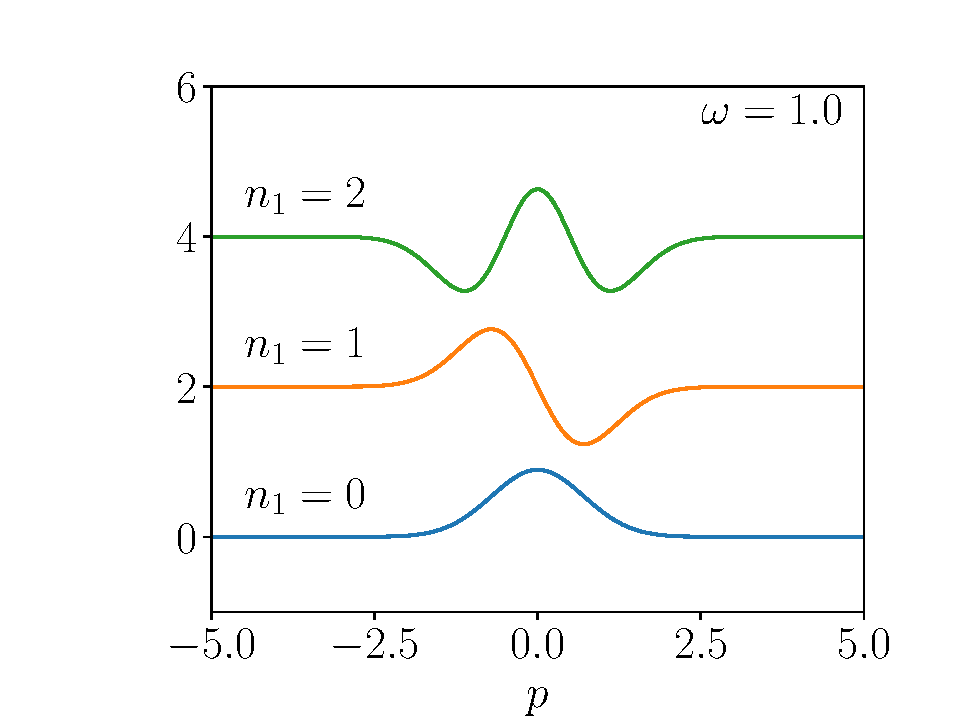
\includegraphics[width=0.5\linewidth]{ho_plot_1}}
\subfloat[\label{fig:ho_wf_w_4}]{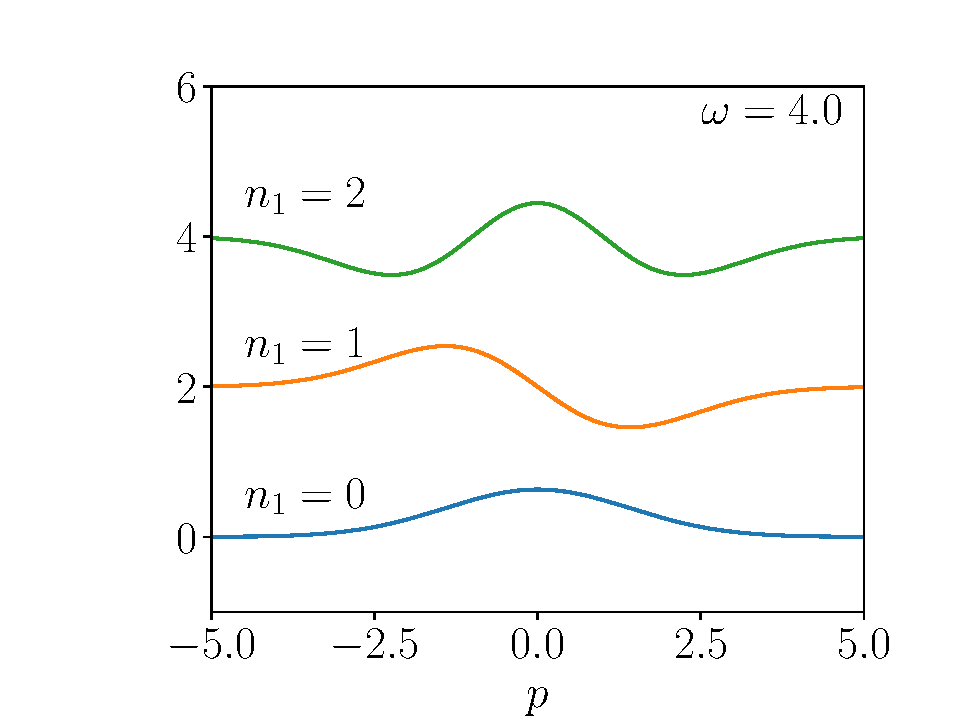
\includegraphics[width=0.5\linewidth]{ho_plot_4}}
\end{center}
\caption{1-dimensional harmonic oscillator wavefunctions for the three lowest energy states for (a) $\omega=1$ and (b) $\omega=4$.}
\label{fig:ho_wf}
\end{figure}

The 1-dimensional harmonic oscillator is a single particle in a purely quadratic potential, $\hat{V}(x) = m\omega^2 \hat{x}^2/2$. The Hamiltonian for the quantum harmonic oscillator is given by
\begin{equation}
\hat{H}_{HO} = \frac{\hat{p}^2}{2m} + \frac{1}{2}m\omega^2\hat{x}^2,
\end{equation}
which has eigenstates $\ket{n}$, which have corresponding wavefunctions
\begin{equation}
\Psi_n(x) = \frac{1}{\sqrt{2^n n!}}\left(\frac{m \omega}{\pi \hbar}\right)^{1/4}e^{-m \omega x^2 / 2 \hbar} H_n\left(\sqrt{\frac{m \omega}{\hbar}}x\right)
\end{equation}
\begin{equation}
\Phi_n(p) = \frac{(-i)^n}{\sqrt{2^n n!}}\left(\frac{1}{\pi m \hbar \omega}\right)^{1/4}e^{-p^2 / 2 m \hbar \omega} H_n\left(\frac{p}{\sqrt{m \omega \hbar}}\right)
\end{equation}
where $H_n(x)$ is the $n$-th Hermite polynomial. The three lowest energy momentum-space wavefunctions, $\Phi_n(p)$, can be seen in Fig.~\ref{fig:ho_wf}. The harmonic oscillator Hamiltonian can also be rewritten as
\begin{equation}
\hat{H}_{HO} = \hbar \omega \left(\hat{a}^\dagger \hat{a} + \frac{1}{2}\right),
\end{equation}
where $\hat{a}^\dagger$ and $\hat{a}$ are raising and lowering operators which act on the harmonic oscillator eigenstates like
\begin{equation}
\hat{a}^\dagger\ket{n} = \sqrt{n + 1}\ket{n+1}
\end{equation}
\begin{equation}
\hat{a}\ket{n} = \sqrt{n}\ket{n-1}.
\end{equation}

For an operator, $\hat{V}$, represented with respect to a momentum basis, $V(p, p')$, a transformation to a harmonic oscillator basis can be achieved by the following calculation:
\begin{equation}\label{eq:ho_transform}
\bra{n}\hat{V}\ket{n'} = \iint V(p, p') \Phi_n^*(p) \Phi_{n'}(p') \,dp\,dp'.
\end{equation}

\subsection{Many-particle states}

For a system of $A$ non-interacting particles, the energy eigenstates of the system can be written as a product of the eigenstates of the single particle Hamiltonians:
\begin{equation}
\ket{\Psi} = \prod_{i=1}^{A}\ket{\Psi_k}_i
\end{equation}
where $\ket{\Psi_k}_i$ is the $k$-th eigenstate of the $i$-th particle's single particle Hamiltonian. For $A$ non-interacting particles in a harmonic oscillator potential, these product states are denoted by:
\begin{equation}
\ket{n_1 n_2 ... n_A} = \prod_{i=1}^{A}\ket{n_i}_i.
\end{equation}


\section{1-Dimensional System of Bosons}

The Hamiltonian for a 1-dimensional system of $A$ identical bosons with mass $m$ that interact via a local two-body potential is as follows:
\begin{equation}
\hat{H} = \frac{1}{2 m} \sum_{i=1}^A \hat{k}_i^2 + \sum_{i=1}^A\sum_{j=i+1}^{A} \hat{V}(x_i - x_j).
\end{equation}
In this equation, the $\hat{k}_i$ are the single-particle momenta and the $x_i$ are the single-particle coordinates. A local potential is a function of the distance between two particles, as opposed to a function of both of their absolute coordinates.

\subsection{Jacobi Coordinates}

A factorization of the Hamiltonian into a center-of-mass component, which is unaffected by the local potential, and a component relative to the center of mass is possible. This is achieved by a transformation to relative momentum Jacobi coordinates \cite{Jurgenson:2008jp}. These are defined to be:
\begin{equation}
p_i = \sqrt{\frac{i}{i+1}} \left(\frac{1}{i} \sum_{j=1}^{i}(k_j - k_{i+1})\right),
\end{equation}
with $k_i$ being the single-particle momenta as mentioned above. It is worth noting that for a system of $A$ particles, we only need $A-1$ Jacobi momentum coordinates. We can get $\hat{V}$ in terms of incoming Jacobi momentum $p$ and outgoing momentum $p'$ by taking the following Fourier transform of $\hat{V}(x_1 - x_2)$
\begin{equation}
\hat{V}(p, p') = \int \hat{V}(\sqrt{2} l_1) e^{- i (p - p') l_1} \,dl_1,
\end{equation}
where $l_1$ is the coordinate conjugate of $p_1$, $(x_1 - x_2)/\sqrt{2}$. Removing the center-of-mass component of the Hamiltonian, we find the new Hamiltonian to be
\begin{equation}
\hat{H} = \frac{1}{2 \mu} \sum_{i=1}^{A-1} \hat{p}_i^2 + \sum_{i=1}^{A-1}\hat{V}(p_i, p_i'),
\end{equation}
where $\mu$ is the reduced mass given by $\mu = m / A$ for particles of equal mass. For the purposes of this work, we will be starting with a potential defined with respect to the Jacobi momentum coordinates, avoiding the process of Fourier transforming a local coordinate-space potential.

\subsection{Transformation To Harmonic Oscillator States}

In momentum space, SRG evolutions require separate treatment of 2-body, 3-body, and higher-body potentials, to avoid delta functions caused by spectator particles \cite{glöckle1983quantum}. A particle is a spectator particle when it is in a state where it does not interact with two particles that are interacting with each other. To avoid the cognitive load of handling all these potentials separately, we can make a transformation to a discrete basis. The discrete basis of choice for this project is the harmonic oscillator basis with respect to the Jacobi coordinates. This transformation can be achieved as shown in Eq.~\ref{eq:ho_transform}. From here on out, $\ket{n_i}$ will mean the $n$-th harmonic oscillator state with respect to the $i$-th Jacobi coordinate. So for a full treatment of an $N$-particle system, we will need product states for $N-1$ Jacobi coordinates,
\begin{equation}
\ket{n_1 n_2 ... n_{A-1}} = \prod_{i=1}^{A-1}\ket{n_i}.
\end{equation}

\subsection{Symmetrizing the Harmonic Oscillator Basis}

According to the spin-statistics theorem, the state of a system of bosons must be symmetric under any permutation of the particle coordinates \cite{streater2000pct}. We approach the problem of generating a basis of states that reflect this symmetry recursively, by first symmetrizing the 2-body system and then going from a symmetrized $(A-1)$-body basis to a symmetrized $A$-body basis. At each stage, we must diagonalize the symmetrizer, the form of which we will show for the 2-body and 3-body cases.

For the 2-particle system, we are only working with the first Jacobi coordinate and the harmonic oscillator states corresponding to it, $\ket{n_1}$. The symmetrizer is $\hat{S} = (1 + \hat{P}_{12})/2$, where $\hat{P}_{ij}$ is the operator that exchanges the coordinates between $i$-th and $j$-th particles. Because harmonic oscillator wavefunctions are either even for even $n$ or odd for odd $n$, $\hat{P}_{12} \ket{n_1} = (-1)^{n_1} \ket{n_1}$ and the symmetrizer is already diagonal with eigenvalue 0 for odd $n_1$ and eigenvalue 1 for even $n_1$. We select the states with eigenvalue 1 to create our symmetric harmonic oscillator basis for the 2-particle system.

To generate the partially symmetrized basis for the 3-body system, we take the states $\ket{n_1 n_2}$ where the possible $n_1$ values come from the symmetrized 2-body basis. The general 3-body symmetrizer is governed by the permutation group $S_3$, generated by $\hat{P}_{12}$ and $\hat{P}_{23}$, and has the form
\begin{equation}
\hat{S} = \frac{1}{6}(1 + \hat{P}_{12} + \hat{P}_{23} + \hat{P}_{23}\hat{P}_{12} + \hat{P}_{12}\hat{P}_{23}\hat{P}_{12})
\end{equation}
Since the states included in our to-be-symmetrized basis are already symmetric with respect to $\hat{P}_{12}$, the symmetrizer simplifies to $\hat{S} = (1 + 2\hat{P}_{23})/3$. The matrix elements of $\hat{P}_{23}$ in our partially symmetrized basis are
\begin{equation}
\bra{n_1' n_2'}\hat{P}_{23}\ket{n_1 n_2} = \delta_{N',N} \bra{n_1' n_2'}\ket{n_1 n_2}_3,
\end{equation}
where $N'=n_1' +n_2'$, $N=n_1 + n_2$, and $\bra{n_1' n_2'}\ket{n_1 n_2}_3$ is the 1-dimensional harmonic oscillator transformation bracket for particles with mass ratio 3. This transformation bracket value is calculated as
\begin{equation}
\bra{n_1' n_2'}\ket{n_1 n_2}_3 = \frac{\sqrt{n_1!n_2!}}{\sqrt{n_1'!n_2'!}}\sum_{k=0}^{n_1'}\binom{n_1'}{k}\binom{n_2'}{n_2 - k}\left(\frac{1}{2}\right)^{n_1' + n_2 - 2k}\left(\frac{\sqrt{3}}{2}\right)^{n_2' - n_2 + 2k} (-1)^{n_2-k}.
\end{equation}
Diagonalizing $\hat{S}$ will give eigenvectors that are normalized linear combinations of product states with the same total harmonic oscillator number $N$. We again select the ones with eigenvalue 1 and keep those as our fully symmetrized 3-body basis. While the project leading up to this thesis only worked with 2-particle and 3-particle systems and thus only the treatment of symmetrizing those bases is relevant to this work, the procedure is generalizable to symmetrize up to any $A$-particle basis. The details of this procedure are explained in Ref.~\cite{Jurgenson:2008jp}.

\subsection{Matrix Elements in the 3-Body Harmonic Oscillator Space}

From Eq.~\ref{eq:ho_transform}, we are able to transform both parts of our 2-body Hamiltonian into the symmetrized 2-body harmonic oscillator basis. In order to work in a symmetrized 3-body basis, we need to compute the kinetic energy for the 3-body system and embed the 2-body potential in the 3-body space. Both the $A$-body kinetic energy and the $A$-body embedded 2-body potential are defined with respect to their $(A-1)$-body counterparts \cite{Jurgenson:2008jp}, so we will set up the discussion to give those formulas. Let $\ket{N_A i_A}$ be a symmetrized $A$-body state with total harmonic oscillator number $N_A$ and degeneracy label $i_A$. $\ket{N_A i_A}$ is defined as
\begin{equation}
\ket{N_A i_A} = \sum_{l=1}^k c_l \ket{N_{A-1} i_{A-1}; n_{A-1}},
\end{equation}
where $k$ is the number of states in the linear combination, the $c_l$ are the coefficients of the linear combination of product states that make up the symmetrized state, $\ket{n_{A-1}}$ is a harmonic oscillator state with respect to the $(A-1)$-th Jacobi coordinate, and $\ket{N_{A-1} i_{A-1}}$ is a symmetrized $(A-1)$-body state. The $A$-body kinetic energy is calculated as
\begin{equation}
\begin{aligned}
\bra{N_A' i_A'}\hat{T_A}\ket{N_A i_A} = & \sum_{l=1}^k \sum_{l'=1}^{k'} c_l c_{l'}' (\bra{N_{A-1}' i_{A-1}'}\hat{T_{A-1}}\ket{N_{A-1} i_{A-1}}\delta_{n_{A-1}',n_{A-1}} \\ 
& - \frac{\omega}{4}\delta_{N_{A-1}',N_{A-1}}(\sqrt{(n_{A-1} + 1)(n_{A-1} + 2)}\delta_{n_{A-1}',n_{A-1} + 2} \\
& + \sqrt{n_{A-1}(n_{A-1} - 1)}\delta_{n_{A-1}',n_{A-1} - 2} \\
& - (2 n_{A-1} + 1)\delta_{n_{A-1}',n_{A-1}})).
\end{aligned}
\end{equation}
Similarly, the embedded 2-body potential in the $A$-body basis is calculated as
\begin{equation}
\bra{N_A' i_A'}\hat{V_A}\ket{N_A i_A} = \frac{A}{A-2} \sum_{l=1}^k \sum_{l'=1}^{k'} c_l c_{l'}' \bra{N_{A-1}' i_{A-1}'}\hat{V_{A-1}}\ket{N_{A-1} i_{A-1}}\delta_{n_{A-1}',n_{A-1}}.
\end{equation}

\section{Similarity Renormalization Group}

The similarity renormalization group (SRG), whose use in low-energy nuclear physics was initially explored at OSU \cite{Jurgenson:2007td}, is one method of reducing the computational complexity of low-energy nuclear calculations. The idea behind it is to continuously unitarily transform the operator of interest (for example, the Hamiltonian) into a simpler form. This simpler form is chosen to allow the large basis to be truncated without affecting the operator eigenvalues, which are essential to the truncated operator's utility in later calculations. The SRG transformation is given by the flow equation for the evolving Hamiltonian $\hat{H}_s$,
\begin{equation}
\frac{d \hat{H}_s}{ds} = [\hat{\eta}_s, \hat{H}_s],
\end{equation}
where $[A, B]$ is the matrix commutator and $\hat{\eta}_s$ is the generator of the transformation which is defined as
\begin{equation}
\hat{\eta}_s = [\hat{G}_s, \hat{H}_s],
\end{equation}
where $\hat{G}_s$ is known as the flow operator. The changes in the Hamiltonian over the course of the SRG evolution are absorbed into the potential, $\hat{V}_s$, leaving the kinetic energy, $\hat{T}$, independent of $s$, the flow parameter. $s$ is taken to be 0 for the un-evolved Hamiltonian. It is often convenient to use $\lambda = 1 / s^{1/4}$ as an alternative flow parameter, so instead of going from $s=0$ towards $s=\infty$ over the course of an SRG transformation, you are going from $\lambda=\infty$ towards $\lambda=0$. For our purposes, $\lambda=40$ (or $s=3.9 \times 10^{-7}$) will be a good enough place to start with the initial Hamiltonian.

\subsection{Induced Many-Body Forces and Flow Operators}

The SRG evolution is fully unitary for an $A$-body operator when done in the $A$-body space. However, working in the full many-body space is only feasible for the smallest of systems, due to the combinatorial scaling of the basis size with respect to $A$. When evolving an $A$-body system operator in some smaller basis, the SRG evolution induces many-body forces which show up as an error when eventually computing operator observables further down the line. This error has limited the SRG's domain of applicability to calculations for small to medium-sized systems.

Certain results have suggested that alternative choices for the flow operator, $\hat{G}_s$, could reduce this many-body force induction and thereby reduce the error induced by applying SRG to calculations \cite{Dicaire:2014fra}. The standard choice for $\hat{G}_s$ is the kinetic energy, which is easy to calculate and represent in most problems. Alternative flow operator choices have been explored previously, but not thoroughly.

\subsection{Value of the 1-Dimensional Laboratory}

SRG was explored initially in the 1-dimensional setting, which made it easy to test and allowed those exploring it to learn a great deal, such as the more careful treatment necessary for $A$-body evolutions in momentum space. Moreover, the setup of the 1-dimensional system is analogous to that of more complex calculations, so the results from the 1-dimensional setting generalize to application of the SRG in 3-dimensional calculations. If there is something to be learned about the connection between flow operator and many-body force induction, it is best comprehensively explored in a simple 1-dimensional problem and then generalized to expensive, difficult 3-dimensional calculations.

In chapter \ref{python_lib}, we will explain the structure of the Python framework designed to make it easy to explore SRG in this 1-dimensional setting.
\chapter{\texttt{srg1d} Python Library}\label{python_lib}

In this chapter, we discuss the design and features of the \texttt{srg1d} Python library. The development of this library was a significant portion of the work that led to this thesis. We will begin by discussing the practical importance of a careful, conscious approach to programming for physics, followed by a review of some programming concepts and terms to facilitate the explanation of the library. We will also speak briefly about the Python programming language and the reasons it was chosen for this project. Then, we will move into the design of the library overall as well as the specific parts. Finally, we will discuss details regarding the implementation and testing the library.

\section{Philosophy of Programming for Physics}

The three principles that guided the programming done for this work are modularization, validation, and abstraction. By writing modular code, we isolate logically independent portions of our project that offer some functionality that is useful on its own. These independent parts can then be applied only to those problems to which they are useful. We can also validate the implementation of these isolated functions, testing them through unit tests or by comparing their results to the results of other implementations. Unit tests are especially useful because they isolate specific use-cases. When changes are made to the codebase, running a comprehensive suite of unit tests can give developers a good idea of what features these changes affected and where they can go to fix the new bugs. Finally, with properly modular code, it is possible to offer logical abstractions that allow the user to avoid thinking about low-level implementation details and work in terms of objects that are relevant to the problem at hand.

These principles are realized by most software engineering projects, where maintainability and collaboration are central concerns. However, we feel that they are equally valuable when developing codebases for physics research, for the same reasons. Projects that follow these principles will allow for easier collaboration and set a solid foundation for projects that are extensions of the current work, in addition to bug detection and identification benefits of the approach.

\section{Review of Programming Concepts}

This review assumes the reader has a basic understanding of programming and aims to explain certain programming concepts and communicate their practical importance. This will better equip readers to understand the rest of the chapter.

\begin{itemize}
    \item \textbf{Classes} are a way for programmers to create complex objects for cases where the programming language basic types (integers, floating point numbers, strings, booleans, arrays) are not enough to meet their needs. A class has some internal data, as well as methods and properties which interact with that internal data. A user can create an object of a class by calling its constructor method. It can interact with the object through its interface.
    \item \textbf{Interfaces} define how a user can interact with an object, through methods and properties. Methods typically change the object in some way or do some significant evaluation of the object internals. Properties allow users to extract certain properties of the object, without changing them.
    \item \textbf{Collections} are classes that contain a bunch of similar objects and define how users can access the objects in the collection. Different variations of collections exist to enforce some conditions on the collection, such as no duplicates or limited ways to access objects in the collection.
    \item \textbf{Indexing} is an operation defined on a collection which allows a user to get any object in the collection by providing the collection the proper index. The simplest example of indexing is a standard array, which most people who have used a programming language have seen.
    \item \textbf{Iterating} on a collection is a way for a user to sequentially access every object in a collection. For a user, accessing objects in a collection via iteration requires the user to know as little as possible about the collection or how to actually access the objects in the collection. Some collections guarantee that the order of the objects accessed via iteration is the same every time as long as the collection is not modified. 
    \item \textbf{Mutability} is the ability of an object to be modified by the user after it is created. Mutable objects (or objects that can change by something the user does) give the user more flexibility in terms of possible functionality, but open the door for potential misuse by the user when properties of the collection are saved by the user, the collection is modified, and those saved properties are not updated to reflect the changes. Immutable objects make sense in cases where the objects should not change, like an array of the days of the week.
    \item \textbf{References} allow multiple objects to have access to the same thing. If the reference to an object is given to two different objects and the first modifies the referenced object, the changes will be reflected in the second object as well. This can lead to difficult-to-manage behavior. As a result, it is good to use references in conjunction with immutable objects, because, in that case, both objects can be sure that the object their reference refers to will never change.
\end{itemize}


\section{A Note on the Python Programming Language}

Python is a dynamically-typed, interpreted, high-level programming language that is used for general-purpose programming. Python is used by many, both inside and outside the sciences, and according to StackOverflow, it has ``a solid claim to being the fastest growing major programming language." Python currently has two supported major versions, Python 2 and Python 3, with Python 2 being supported for developers unable to immediately transition to Python 3.

Although the numerical libraries in Python are quite fast due to their low-level C bindings, Python is still not a high-performance language. Projects written in Python that are not satisfied with their performance can profile their code to identify bottlenecks and take advantage of Python bindings to low-level languages like C and Fortran to speed up work-intensive portions of their program. The Pareto principle applied to programming states that 80\% of the work of a program will be done by 20\% of the code, which we call the work-intensive part of the code. A profiling tool like \texttt{cProfile} can be used to help the developer identify these portions. Python's C implementation, Cython, has native C bindings that allow developers to call C subroutines, which will allow them to achieve their desired performance.

However, despite the general computational challenge faced by nuclear theory in general, the simple 1-dimensional system explored here is numerically relatively simple. Thus, high throughput and efficient memory usage are not requirements for these calculations to be done in a reasonable amount of time on any modern personal computer. In addition, Python is extremely expressive with a large standard library and well-documented third party libraries, making developer productivity very high. This was a priority in this research, leading to the decision to work in Python.

The next section discusses the general design of the library and references the interfaces for various different classes. A feature of Python is that users with sufficient knowledge of the internal representation of data in Python classes can directly access those internals and use or modify them how they see fit. This means that published interfaces don't truly limit what a user can do with a library and things like immutability are difficult or impossible to truly enforce. However, Python developers have the philosophy that all Python users are ``consenting adults." This means that the documentation of interfaces and conditions on the objects like immutability are communicated to users in an understanding that they should stick to these documented designs if they expect things to work as advertised.

\section{Library Design}

The class-based abstractions offered by the library offer consistent representations of different logical classes of objects present in any SRG calculation. By offering the user classes and functions that handle much of the complex, but frequently required functionality in any SRG calculation, the library allows the user to focus on exploration and research rather than reinventing the wheel. Behind the abstractions in the library are also several checks that ensure the physical correctness and consistency of what the user is doing. This further boosts user productivity, as the library provide transparent clear errors as to what conditions were not met, allowing the user to quickly understand where the error in their program is.

\begin{figure}[t]
\begin{center}
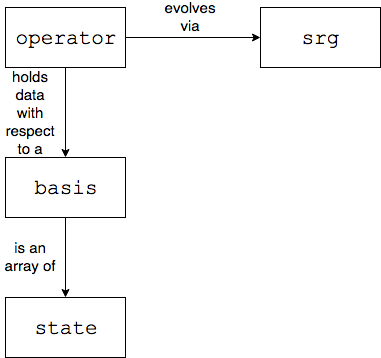
\includegraphics[width=0.6\linewidth]{srg1d}
\end{center}
\caption{A general structure for the modules in the \texttt{srg1d} library.}
\label{fig:srg1d}
\end{figure}

The library is roughly split into two logical halves. The data representation half (\texttt{state}, \texttt{basis}, and \texttt{operator}) handles the representations of the matrices for the operators in the calculations. Its primary goal is to add the context to the numerical representation of matrices and as a result make transformations of those matrices easier to achieve. The evolution half of the library (\texttt{srg}) handles the SRG transformation of the data. While the data representation classes correspond to concrete objects, the \texttt{srg} class is more of a state machine that allows the user to put some data in, turn the crank, and get out intermediate and final results.

\subsection{\texttt{state}}

The \texttt{state} module provides the fundamental building blocks for the data representation side of the library. It contains two classes, \texttt{ho\_state\_2body} and \texttt{ho\_state\_nbody}, that implement the same simple interface. The interface for both classes simply defines a constructor and \texttt{val}, a method to evaluate the harmonic oscillator wavefunction that the state corresponds to at some momentum. These classes are intended to add context data (harmonic oscillator number, number of particles, dirac notation) to the wavefunction that will simplify the evaluation of the wavefunction and allow for the construction of states with more complex structures due to additional physical conditions imposed on the states, like symmetry. Because these states are only intended to be used to get wavefunction values, their interface defines them to be immutable.

\texttt{ho\_state\_2body} represents a 2-body harmonic oscillator state. \texttt{ho\_state\_nbody} is different from \texttt{ho\_state\_2body} in that it represents a general linear combination of $n$-body product states. The only conditions on this linear combination of product states are that it is normalized and that the total harmonic oscillator number for each product state in the linear combination is the same. \texttt{ho\_state\_2body} is the basic building block of these general $n$-body product states.

It is worth mentioning that \texttt{ho\_state\_nbody} does not enforce any symmetry on these states. The conditions imposed on the linear combination of product states are the minimum conditions for such a state to be physically useful. The burden of ensuring proper symmetry falls on the operations creating the states, which is handled elsewhere in the \texttt{srg1d} library. Thus, for the purposes of an SRG calculation, a user should never have to deal with the \texttt{state} module directly.

\subsection{\texttt{basis}}

The \texttt{basis} module provides a basic interface for a \texttt{basis} class and two classes, \texttt{p\_basis} and \texttt{ho\_basis}, that implement this interface. The \texttt{basis} class interface comprises only a constructor, but it also defines \texttt{\_\_len\_\_}, giving the size of the basis, and \texttt{\_\_getitem\_\_}, allowing the user to access a state by its index. These additionally defined methods make any basis indexable and iterable, with iterability being especially valuable for working with bases. The classes that implement the \texttt{basis} interface are also defined to be immutable, because after construction these bases have certain properties (symmetry, completeness, etc.) that would be disturbed by the removal, addition, or modification of a state in the basis.

\texttt{p\_basis} is the representation of a momentum basis. Strictly speaking, a momentum basis is a continuous basis, that is operators need to be defined for any pair of real momenta. However, for numerical purposes, it makes sense to discretize the momentum space and impose some upper and lower cutoffs on momenta included in the basis. The upper and lower cutoffs on a discretized momentum basis are left to the user, who can judge what the range of relevant momenta is. The discretization scheme for the points between those upper and lower bounds is given by a Gaussian quadrature, which provides points $p_i$ and weights $w_i$ at which to evaluate the function. This provides us with the momentum basis for a single Jacobi momentum. From the single momentum basis, we can generate the two Jacobi momentum basis by taking the Cartesian product between two single momentum bases, with the weight assigned to to each new state being the product of the two weights corresponding to the states in the ordered pair. This approach can be used to generate a basis for any number of Jacobi momenta. The data representation of the $n$-body momentum basis is simply a list of these states, which are represented as $n$-tuples with $n-1$ Jacobi coordinates and finally a weight for the state.

\texttt{ho\_basis} is the representation of a harmonic oscillator basis. This is simply a list of harmonic oscillator states (2-body or $n$-body) up to some maximum total harmonic oscillator number, $N_{max}$. The standard constructor for \texttt{ho\_basis} generates a basis of 2-body states with proper symmetry. \texttt{ho\_basis} has a second constructor \texttt{ho\_basis.from\_basis} that takes any $n$-body \texttt{ho\_basis} object and generates an appropriately symmetrized $n+1$-body basis. Additionally, each $n$-body basis has a reference to the $n-1$-body basis used to generate it, which is useful for functions which need to recurse down to the 2-body basis. Because generating bases with appropriate symmetry is an expensive operation, it is important to avoid recreating \texttt{ho\_basis} objects. Thus, the \texttt{srg1d} library makes an effort to work with references to existing objects whenever it is possible.

\subsection{\texttt{operator}}

The \texttt{operator} module provides a simple \texttt{operator} class which couples a matrix with a basis that corresponds to its representation along with several additional useful methods that work on operators. The packaging of a matrix and a basis into one object reduces the potential for bugs when calling methods that require both the data and the basis, which occurs frequently in the setup of an SRG calculation. It also ensures that methods requiring operators can be certain that the basis and matrix are consistent, so methods do not need to do redundant checks, such as ensuring the basis and data sizes match.

The methods provided by the \texttt{operator} module do one of three things: generate operators, transform operators, or embed operators. The operator generating methods, \texttt{create\_ho\_basis\_kinetic\_energy}, \texttt{create\_p\_basis\_kinetic\_energy}, and \texttt{create\_kinetic\_energy}, are methods that calculate the kinetic energy operator in a certain basis and return a corresponding \texttt{operator} object. While the general $n$-body kinetic energy can be calculated directly, the $n$-body kinetic energy is calculated recursively, with the 2-body kinetic energy being the base case. This is where the $n$-body \texttt{ho\_basis} internal reference to the $n-1$-body \texttt{ho\_basis} comes in handy.

The \texttt{transform\_operator\_to\_p\_basis}, \texttt{transform\_operator\_to\_ho\_basis}, and \texttt{transform\_operator} methods all compute a unitary transformation for the operator data between a harmonic oscillator basis representation and a momentum basis representation. The harmonic oscillator basis has a parameter $\omega$ which relates to the strength of the oscillator; this value needs to be optimized for the transformation from momentum space to harmonic oscillator space. If no value is given for $\omega$ in the function call, it will be optimized internally and return with the transformed operator. A transformation from harmonic oscillator space to momentum space requires the $\omega$ used originally to transform the operator to harmonic oscillator to be passed in by the user. A future implementation may add an internal member to the \texttt{operator} class keeping track of $\omega$ for operators in harmonic oscillator space to avoid placing the burden of keeping track of the value on the user.

Finally, \texttt{embed\_operator} embeds an operator in harmonic oscillator space in a higher-body harmonic oscillator basis provided by the user. The logic for this embedding is similar to the logic for generating the general $n$-body kinetic energy in harmonic oscillator space. Again, this algorithm takes advantage of the internal reference to the $n-1$-body basis kept by the $n$-body \texttt{ho\_basis} to avoid recreating a new equivalent basis.

\subsection{\texttt{srg}}

The \texttt{srg} module only contains the \texttt{srg} class, which handles the evolution of some operator via the SRG flow equation. The three methods of this class are its constructor, \texttt{evolve}, and \texttt{set\_generator}. The constructor takes in a potential and a kinetic energy (which are the Hamiltonian when added up), as well as a 2-tuple of matrices called the generator. These two generator matrices are weights assigned to matrix elements of the potential and kinetic energies that are used when computing the flow operator $G_s$. For the standard $G_s = T_{rel}$, a zero matrix for the generator corresponding to the potential energy and a matrix of ones for the generator corresponding to the kinetic energy is one way to compute the correct flow operator. Allowing the user to provide a function to compute the flow operator from the kinetic and potential energy was a design that was considered, but rejected in favor of the easier-to-check and less complex generator matrices. The \texttt{set\_generator} method allows the user to alter the flow operator used between evolutions. While it is not typically useful to change flow operators part of the way through a full SRG calculation, this was added to allow us to easily switch between operators during calculations and investigate how composite SRG evolutions affect results.

The \texttt{evolve} method evolves the Hamiltonian provided in the constructor to a specified value of the flow parameter $\lambda$. The method uses \texttt{scipy.integrate.ode} to solve the system of coupled differential equations. In addition to taking the target value of $\lambda$ as a parameter, it also optionally takes parameters to specify an integrator and parameters for that integrator for users with specific needs who are also familiar with the integrators available through the \texttt{scipy.integrate.ode} method. The default integrator used is \texttt{\'dopri5\'}, a fourth order Runge-Kutta method that works well for non-stiff systems. However, for problems that are more stiff, it makes sense to switch to \texttt{\'lsoda\'}, a solver that dynamically switches between different algorithms for non-stiff and stiff problems. The only downside to the \texttt{\'lsoda\'} integrator is that it is not re-entrant meaning that different \texttt{srg} objects cannot both use it at the same time and therefore would be unable to run in parallel. The \texttt{srg} class also has accessor functions to allow the user to quickly access the data of the evolved potential as well as the current value of the flow parameter $lambda$.

\section{Implementation}

The first version of the library was written to be compatible only with Python 2.7. We made a decision fairly early on to focus development on Python 3, with an auxiliary goal of still being Python 2 compatible. Over time, the attention paid to keeping the code Python 2 compatible waned. As a result, it is currently not able to be used in Python 2. Fortunately, the recent Python Developers Survey 2017 published by Jetbrains shows that Python 3 is used by 75\% of Python developers as their primary version of the language, a substantial shift from 2013, when this project began, and 2015, when the switch to Python 3 on the project was made. Additionally, Python 2 will officially stop being supported in 2020. All of this leaves the \texttt{srg1d} library in a good place considering Python 3 adoption trends and the waning support for Python 2.

\subsection{Libraries Used}

The only non-standard libraries used in \texttt{srg1d} are NumPy and SciPy. NumPy arrays are convenient for representing vectors and matrices and can be used interchangeably with lists and lists of lists. Additionally, they allow for efficient numerical calculations and are the standard representation for data throughout the NumPy and SciPy libraries. NumPy also offers matrix and vector operations. SciPy extends the utility of NumPy by offering more linear algebra functions such as eigenvalue decomposition and numerical solvers for systems of coupled differential equations. Both NumPy and SciPy are available in the Python Package Index (PyPI) and can be installed easily with the Python package management system, \texttt{pip}.

\subsection{Handling Unexpected Usage}

It was mentioned previously that Python relies on library implementers and library users being ``consenting adults." As far as libraries are concerned, this means library implementers only have an obligation to document the interface, not actually enforce it. This is different from programming in languages like C++ or Java, where static typing forces users to adhere to an interface. In fact, Python users typically take the stance that if a library user is able to provide an object that doesn't strictly match the library interface but interacts with the library implementation in a way that works, that usage is fine. This is known as ``duck typing," following the principle ``if it walks like a duck and talks like a duck, then it must be a duck." In keeping in line with this philosophy, the \texttt{srg1d} library never enforces the type of objects using \texttt{isinstance}. Instead, it typically checks that an object implements the necessary interface, which is done by checking the existence of the required methods and properties.

However, in cases where data is taken in but not used, like in an object constructor call, it makes sense to ensure that errors that will definitely lead to problems later are immediately detected and pointed out to the user. Examples of this include checking that matrices that will be multiplied later have the correct dimensions and checking that corresponding bases and matrices have the same length. The implementation of the \texttt{srg1d} library strives to do comprehensive checks in this regard wherever it is reasonable, primarily in object constructors.

One notable exception to this rule is the \texttt{val} method from the \texttt{ho\_state\_2body} and \texttt{ho\_state\_nbody} class. This method is ideally never directly called by the user, but profiling done with \texttt{cProfile} showed that around 75\% of time spent initializing the SRG calculation (calculating operators and transforming or embedding them) was spent inside of it. Removing the checks done on the parameters in \texttt{val} halved the time spent inside it. Outer loop optimizations also reduced the number of calls to the method from several million to several hundred thousand. As the library is designed to make it so the user never has to use this method and it is so frequently called, we believe removing error checking from it is worth the performance. In cases where the user does need to directly work with the \texttt{ho\_state\_2body} and \texttt{ho\_state\_nbody} objects, they still have the documentation of the interface to fall back on.

\section{Testing}

An effort was made to adopt a test-driven development (TDD) approach in the development of the \texttt{srg1d} library. Tests are written using the \texttt{unittest} standard Python library, and the documented way to run the tests involves using \texttt{nose}. \texttt{nose} is an extension to \texttt{unittest} that can easily be installed via \texttt{pip}. The installation of \texttt{nose} comes with a script called \texttt{nosetests}, which can be run by the user and will automatically discover and run tests. While the project does not have complete code coverage, the existing tests focus on object constructors and specifically on graceful failure when these constructors are incorrectly called. The \texttt{state} module has good test coverage of the \texttt{val} method for both classes. One of the goals for the library before publication of the package is to extend the current incomplete test suite to have better coverage.



\chapter{Approach to Exploration}\label{methods}

In this chapter, we discuss the approach taken to reproducing results from previous work and exploring how using alternative flow operators changes these results.

\section{Objectives}

\subsection{Verify Many-Body Force Induction}

The first major goal of the project was to use the new, more flexible framework provided by the \texttt{srg1d} library to reproduce 2-body and 3-body results published in Ref.~\cite{Jurgenson:2008jp}. While the 2-body results do not give any insight into many-body force induction, they offer an intermediate point for us to look at and be certain of the correctness of our work so far. The 3-body results allow us to look at many-body force induction and reproducing the Jurgenson 3-body results gives us a good point to compare to when testing other flow operators.

\subsection{Test Alternative Flow Operators}

The second major goal after reproducing previous results was to use alternative flow operators and observe how the results of the SRG evolution change. With the framework of the \texttt{srg1d} library, changing the flow operator for existing an SRG calculation is as simple as changing two lines of code in most cases. With the ability to easily switch flow operators, we are able to easily take calculations reproducing previous results and use them with new flow operators to directly see the change caused by changing the flow operator.

\section{2-Particle Systems}

We use the Negele 2-body potential adopted from Ref.~\cite{Alexandrou:1988jg}, which was also used in Ref.~\cite{Jurgenson:2008jp}:
\begin{equation}\label{eq:negele}
\hat{V}(p, p') = \frac{V_1}{2\pi\sqrt2}e^{-(p-p')^2\sigma_1^2/8} + \frac{V_2}{2\pi\sqrt2}e^{-(p-p')^2\sigma_2^2/8}.
\end{equation}
We use the same sets of parameters as used previously, detailed in Table \ref{table:negele_params}. The $\hat{V}_\alpha$ potential features a mid-range attraction and a strong short-range repulsion, similar in nature to real nucleon-nucleon potentials. The $\hat{V}_\beta$ potential is a purely attractive potential.

\begin{table}[t]
\begin{center}
\begin{tabularx}{\textwidth}{ X X X X X X X } 
 \hline
 Name & $V_1$ & $\sigma_1$ & $V_2$ & $\sigma_2$ & $E_2$ & $E_3$ \\ 
 \hline
 $\hat{V}_\alpha$ & 12.0 & 0.2 & -12.0 & 0.8 & −0.920 & -2.567\\ 
 $\hat{V}_\beta$ & 0.0 & 0.0 & -2.0 & 0.8 & -0.474 & -1.708 \\ 
 \hline
\end{tabularx}
\end{center}
\caption{Parameters for two variants of the 2-body Negele potential from Eq. \ref{eq:negele} and their corresponding 2-body and 3-body ground state energies, denoted by $E_2$ and $E_3$ respectively.}
\label{table:negele_params}
\end{table}

We compute the 2-body Hamiltonian with this potential in momentum space and verify that the ground state energy eigenvalues match. We then run the SRG method on the 2-body momentum-space Hamiltonian and verify that it is truly unitary and behaves in the same way as in Fig.~\ref{fig:jurg_2body_ev}. We then perform the transformation to symmetrized 2-body harmonic oscillator basis, checking that the ground state energy is unchanged by the unitary transformation. We perform an additional check on the correctness of the transformation by ensuring that the transformed kinetic energy operator is equal to the 2-body kinetic energy as calculated directly from the harmonic oscillator basis.

\begin{figure}[t]
\begin{center}
 \includegraphics*[height=1.4in]{V_srg_lam_40}
\includegraphics*[height=1.4in]{V_srg_lam_5}
 \includegraphics*[height=1.4in]{V_srg_lam_3}
 \includegraphics*[height=1.4in]{V_srg_lam_2}
\end{center}
\caption{Evolution from $\lambda=\infty$ to $\lambda=2$ of the even part of the $\hat{V}_\alpha$ potential in 2-body momentum space from Ref.~\cite{Jurgenson:2008jp}. Figure reproduced with permission of the author.}
\label{fig:jurg_2body_ev}
\end{figure}

We then use the 2-body Hamiltonian to experiment with different flow operators. While the 2-body system does not give any insight into the many-body forces induced by SRG when using these flow operators, it does give an excellent way to visualize how the action of the SRG transformation on the operator changes because of the alternative flow operators.

\section{3-Particle Systems}

Moving to a 3-body system allows us to get our first results for 3-body force induction for Hamiltonians evolved in a 2-body system. To observe this, we first generate the 3-body symmetrized harmonic oscillator basis by generating all possible product states, computing and diagonalizing the symmetrizer, and keeping states with eigenvalue 1. With the symmetric 3-body basis, we are able to compute the 3-body kinetic energy and embed the 2-body potential from the 2-body basis in the 3-body basis. With these 3-body operators, we are able to compute the 3-body ground state energy and compare it to the previously published value for it given in Table \ref{table:negele_params}.

\begin{figure}[t]
\begin{center}
\subfloat[$\hat{V}_\alpha$\label{fig:jurg_va}]{\centering\includegraphics*[height=2.5in]{Ebind_3N_Va}}
\hfill
\subfloat[$\hat{V}_\beta$\label{fig:jurg_vb}]{\centering\includegraphics*[height=2.5in]{Ebind_3N_Vf}}
\end{center}
\caption{Demonstration of an induced 3-body force in (a) the 3-body $\hat{V}_\alpha$ ground state energy and (b) the 3-body $\hat{V}_\beta$ ground state energy from Ref.~\cite{Jurgenson:2008jp}. Figure reproduced with permission of the author.}
\label{fig:jurg_vfull}
\end{figure}

After properly embedding the 2-body potential in the 3-body basis, we are able to see how the 2-body SRG evolution with the standard kinetic energy flow operator induces a 3-body force in the 3-body ground state energy. We verify that this behavior matches that shown in Fig.~\ref{fig:jurg_vfull}. We then use the same approach to see the strength of 3-body forces induced by 2-body SRG evolution with alternative flow operators.


\chapter{Results}\label{results}

In this chapter, we discuss the results found through the approach outlined in Chapter \ref{methods}. We see that our results match the results published in Ref.~\cite{Jurgenson:2008jp}. We also note the different behavior of the SRG method when used with alternate flow operators.

\section{2-Body}

For the 2-body momentum-space system, the key results for us to reproduce are the 2-body ground state energies in Table \ref{table:negele_params} and the behavior of the SRG using $\hat{G}_s=\hat{T}$ as shown in Fig.~\ref{fig:jurg_2body_ev}. After transforming to the symmetric 2-body harmonic oscillator basis, we can validate our implementation by showing that the 2-body ground state energies are unchanged and the transformed kinetic energy matches the kinetic energy computed directly from the harmonic oscillator basis.

\subsection{Momentum Space SRG}

\begin{figure}[th!]
\begin{center}
\subfloat[$\hat{G}_s=\hat{T}$\label{fig:2body_T_gen}]{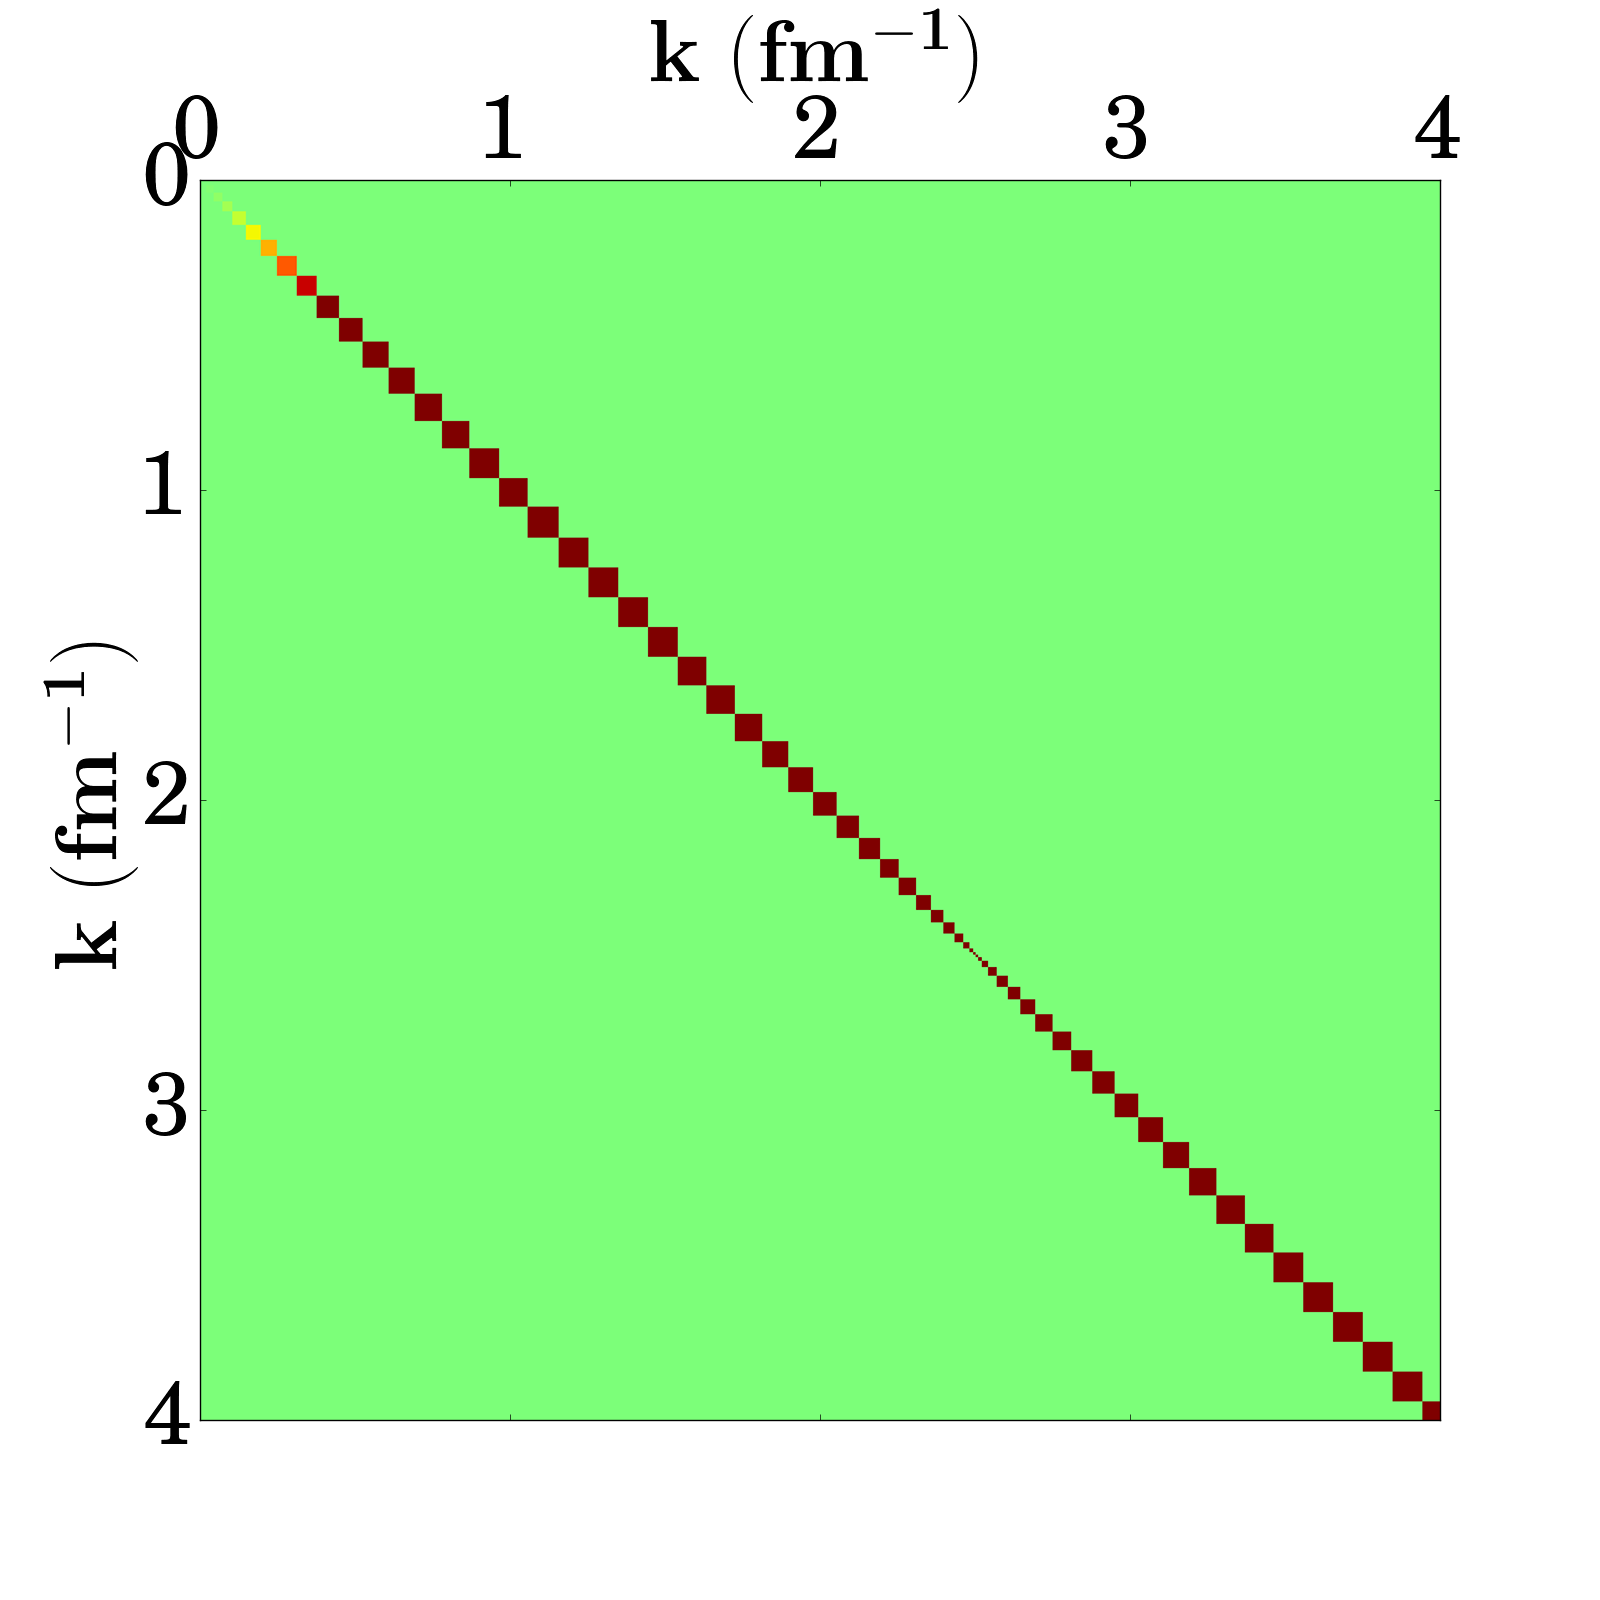
\includegraphics[trim={0 3cm 0 0},clip,width=0.25\linewidth]{T_generator}}
\subfloat[Evolution of $\hat{V}_s$\label{fig:2body_T_ev}]{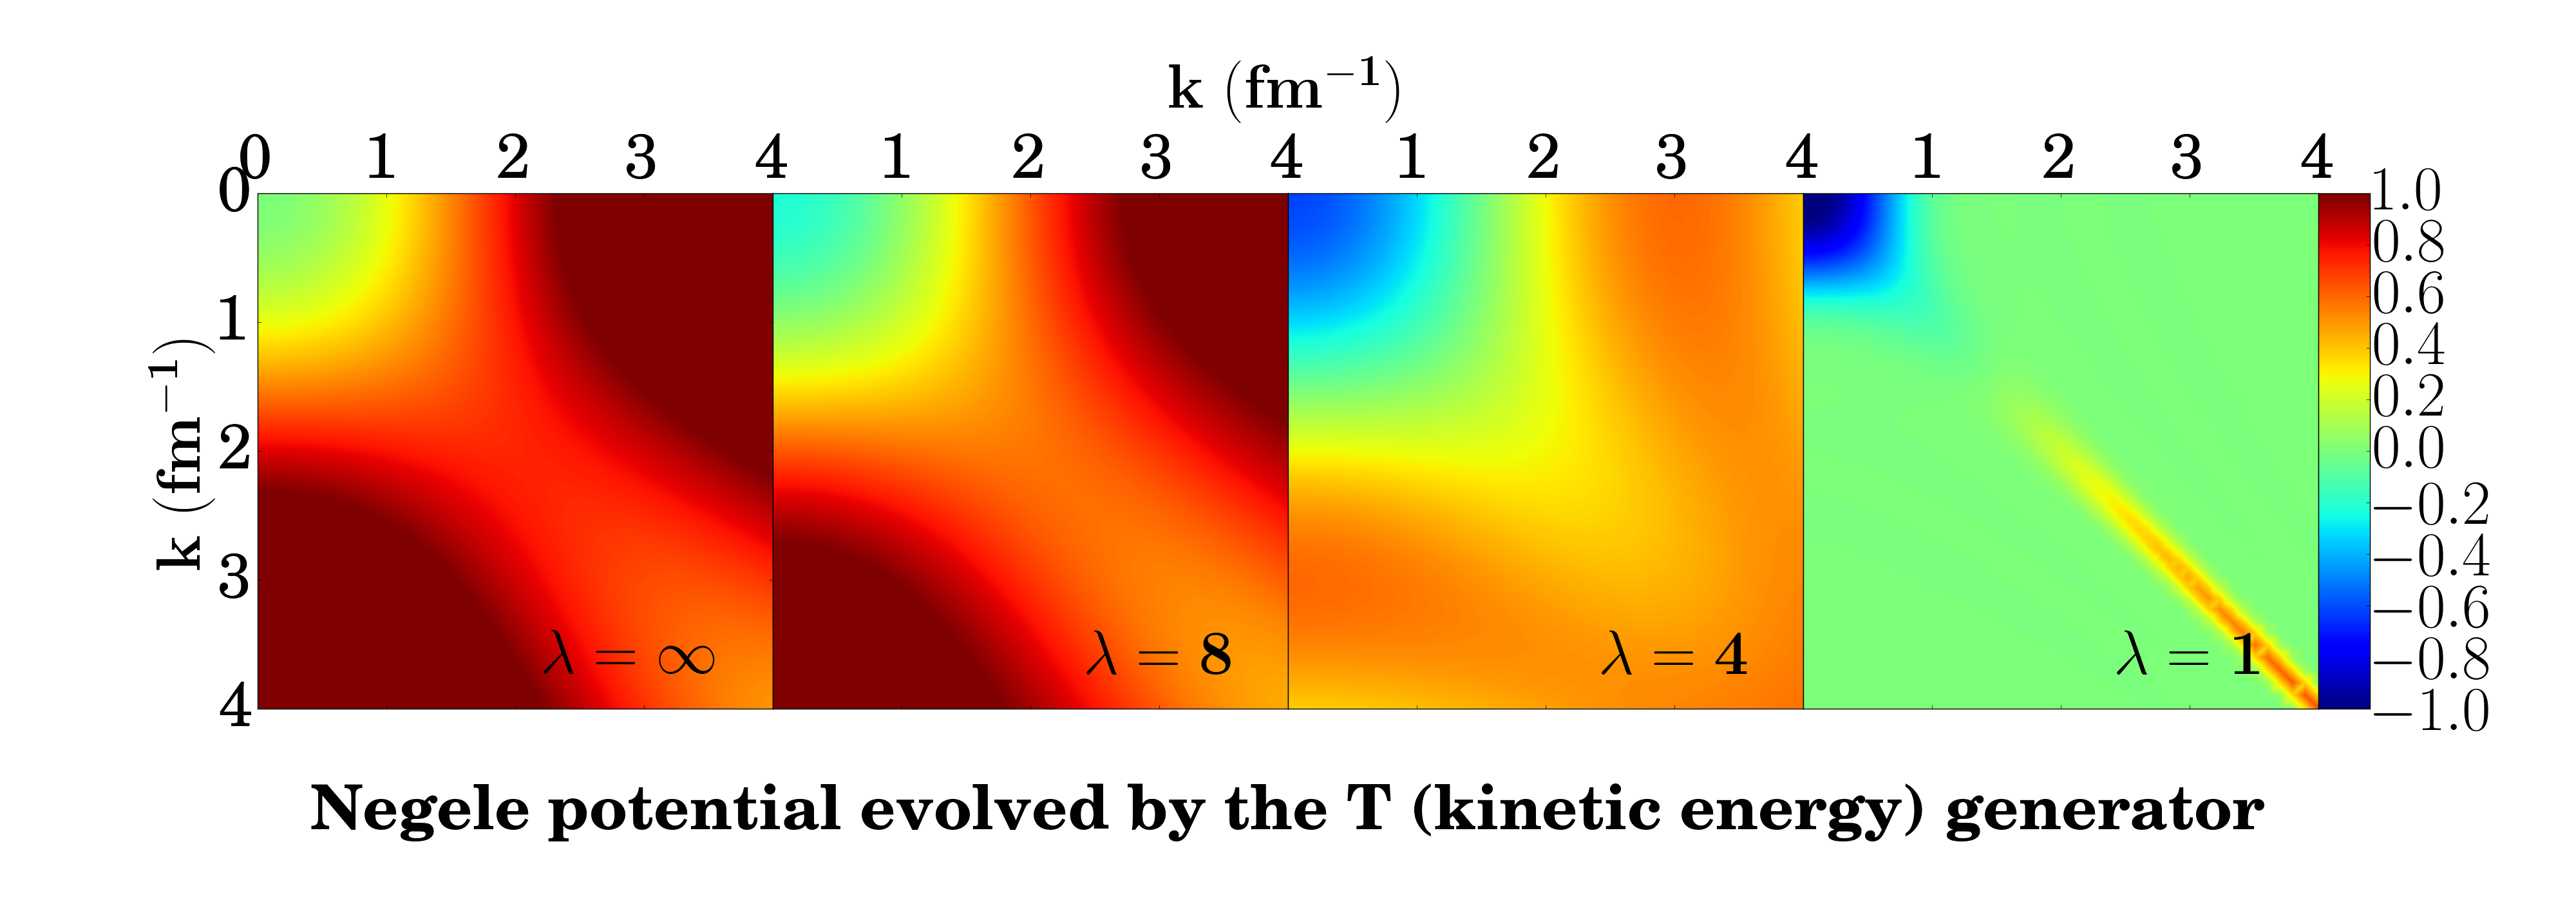
\includegraphics[trim={0 5cm 0 0},clip,width=0.75\linewidth]{T_evolution}}
\end{center}
\caption{Evolution from $\lambda=\infty$ to $\lambda=1$ of the even part of the $\hat{V}_\alpha$ potential in 2-body momentum space with $\hat{G}_s=\hat{T}$ as shown in (a).}
\label{fig:2body_T_full}
\end{figure}

\begin{figure}[th!]
\begin{center}
\subfloat[$\hat{G}_s=\hat{H}_{BD, s=0}$\label{fig:2body_BD_gen}]{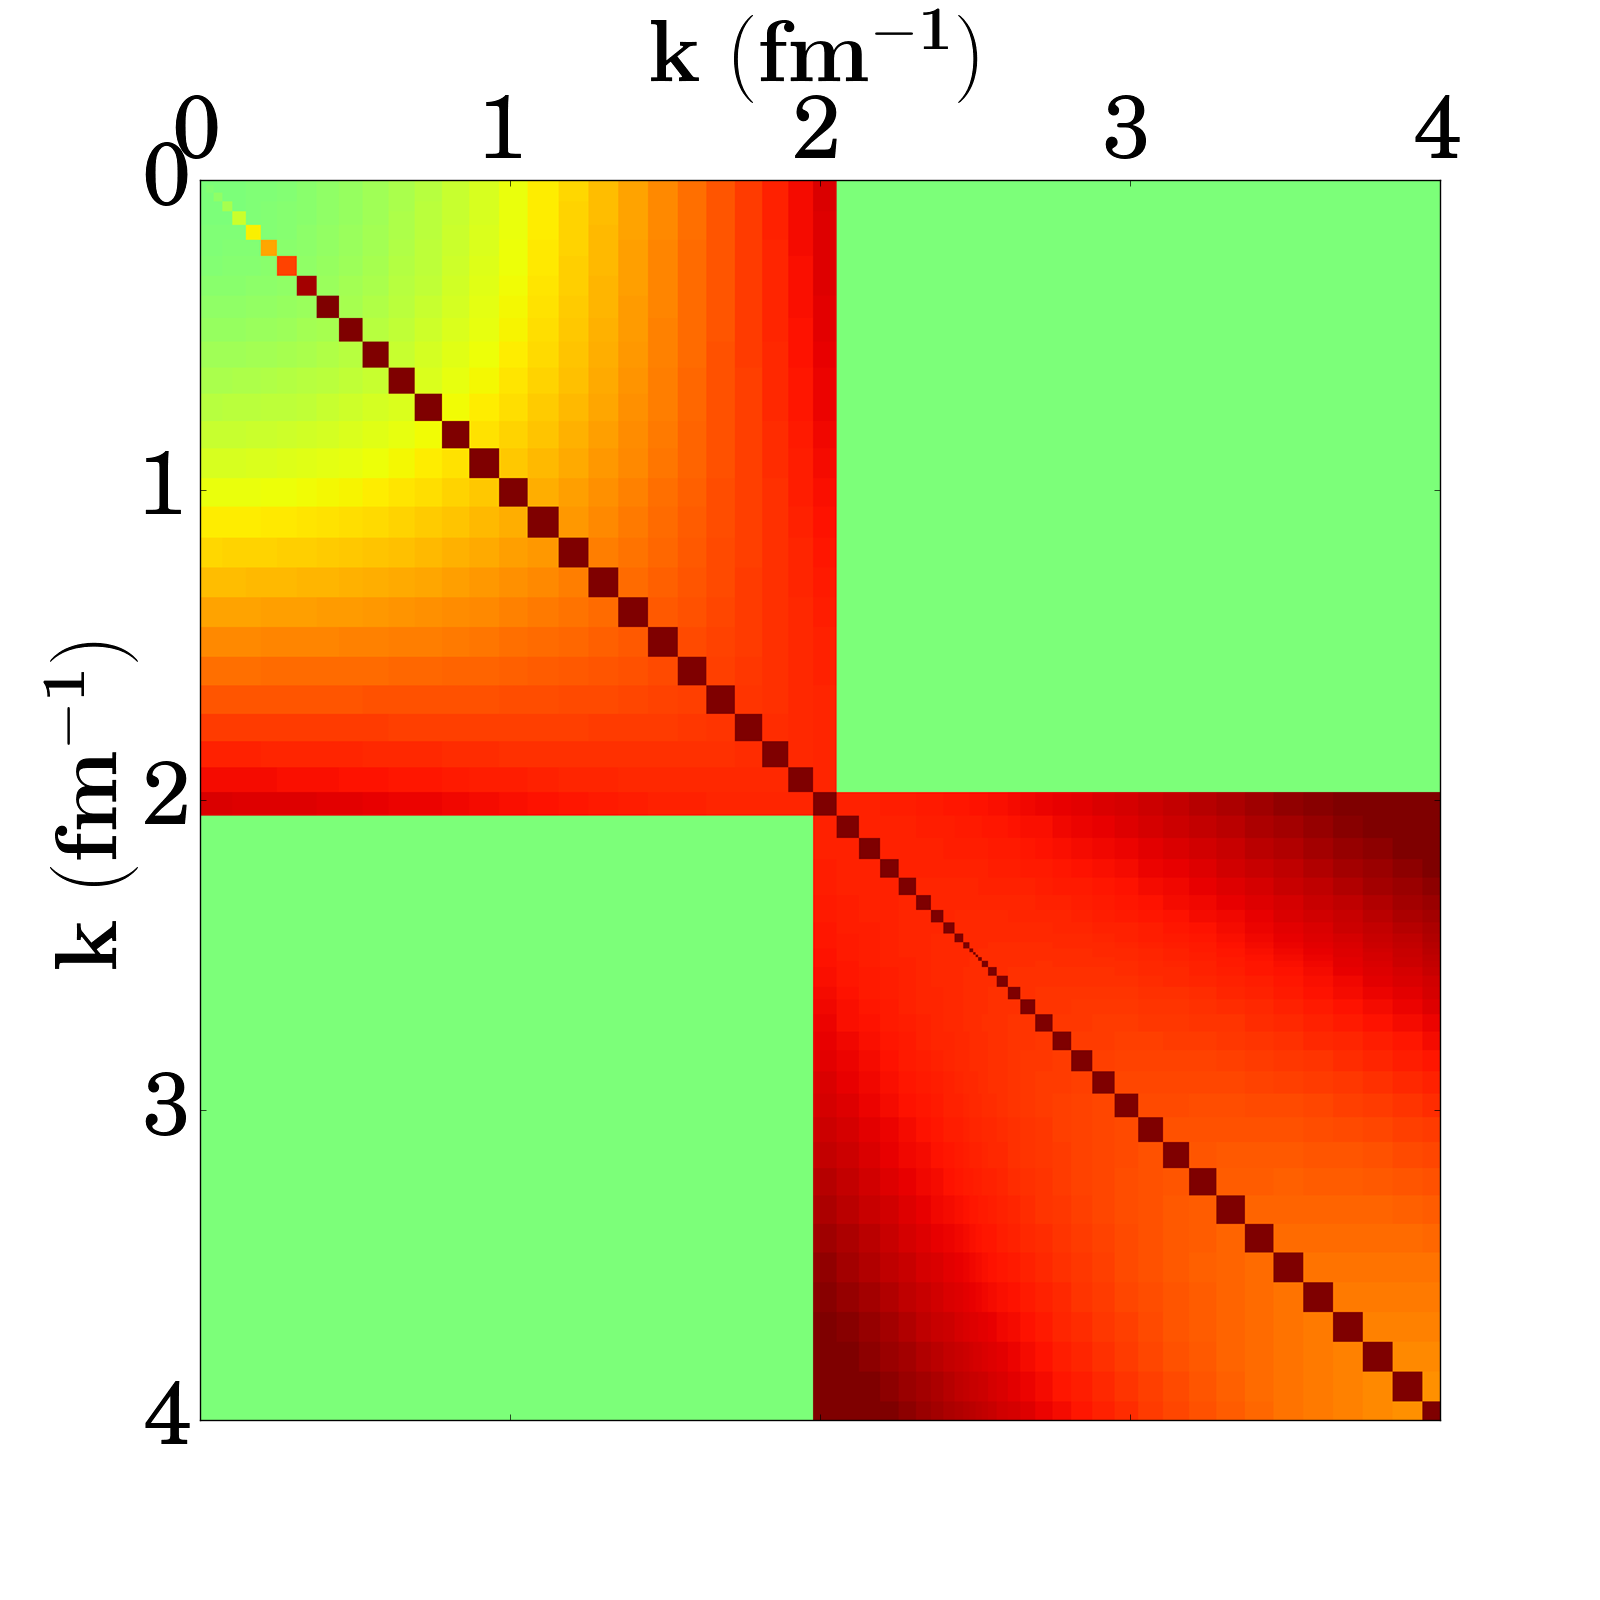
\includegraphics[trim={0 3cm 0 0},clip,width=0.25\linewidth]{BD_1_generator}}
\subfloat[Evolution of $\hat{V}_s$\label{fig:2body_BD_ev}]{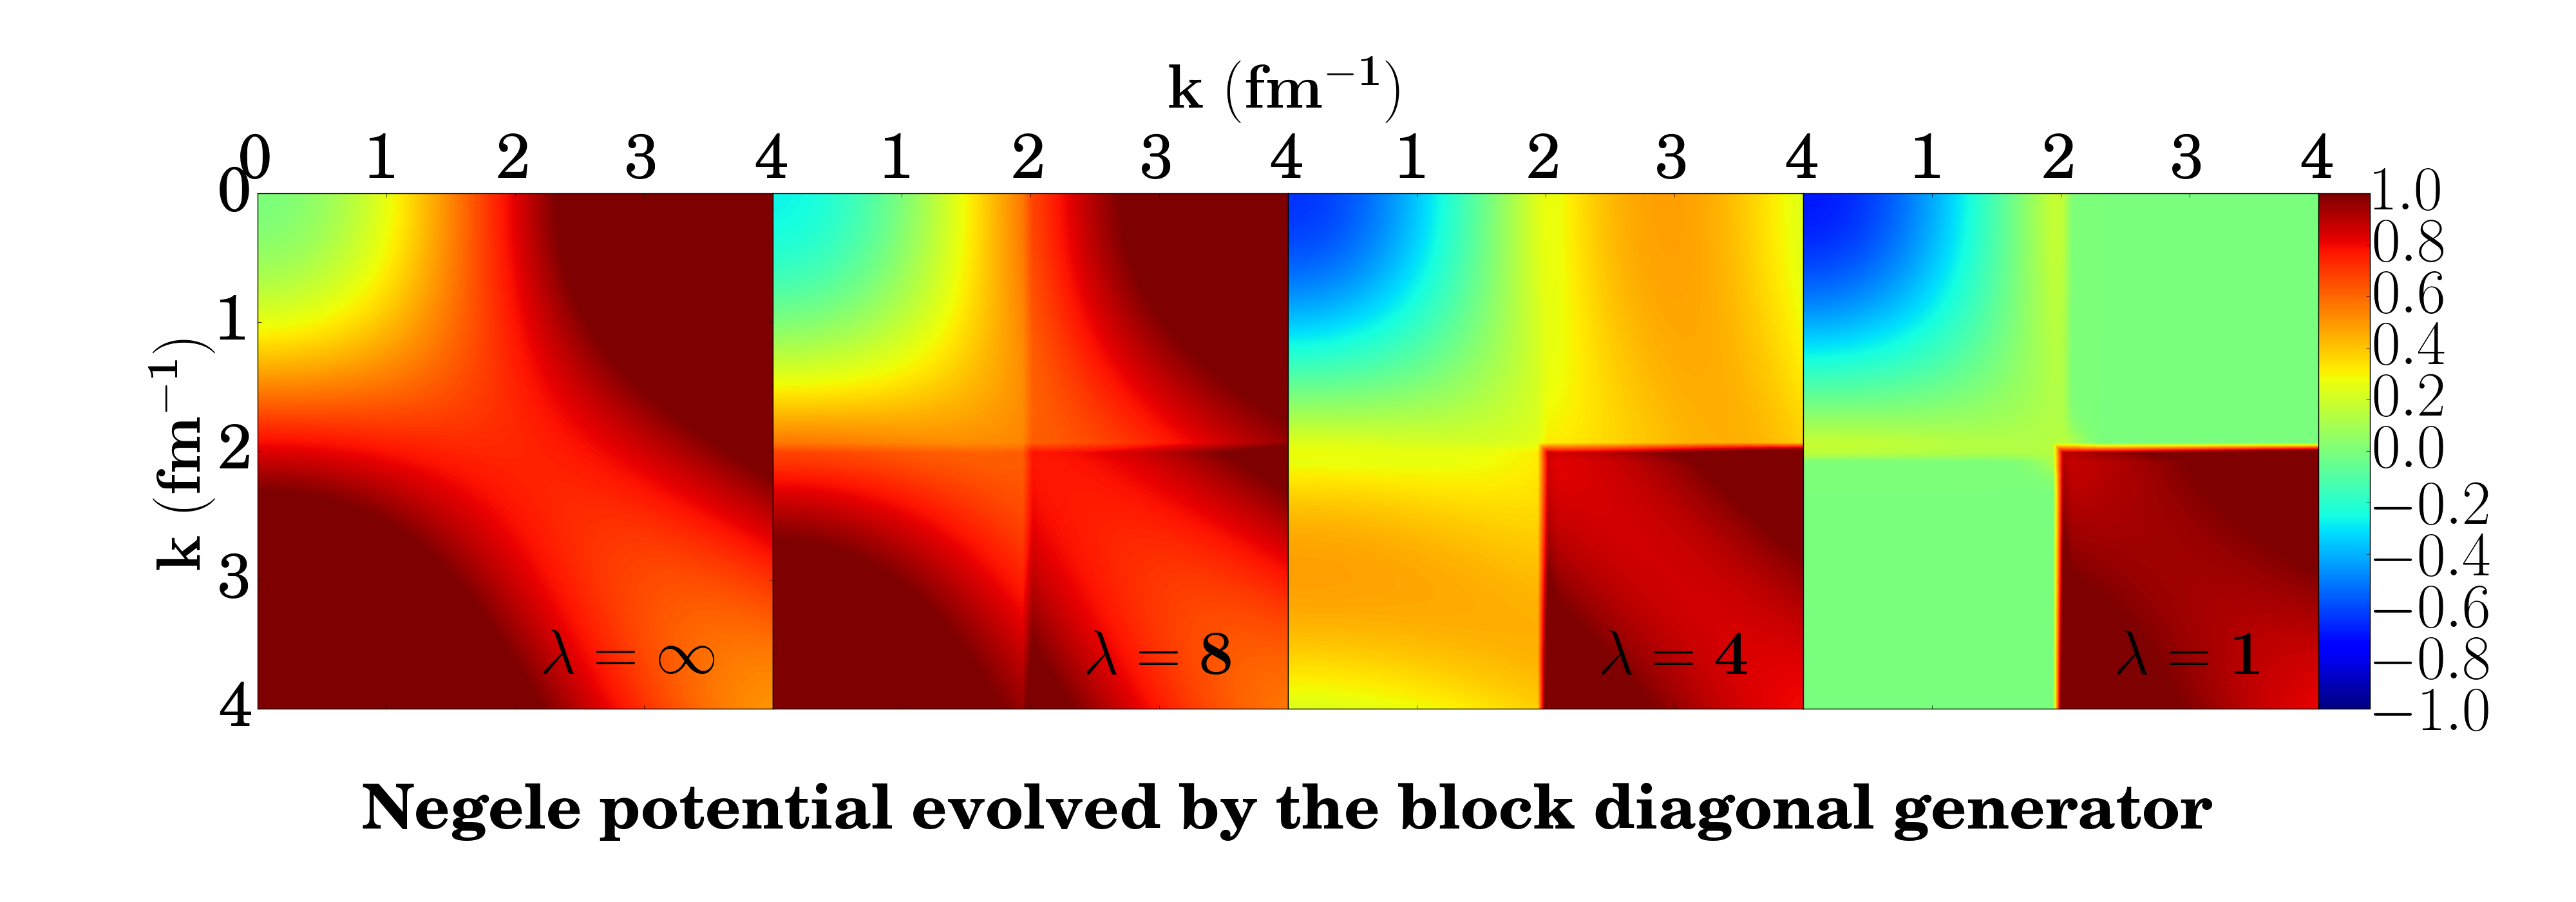
\includegraphics[trim={0 5cm 0 0},clip,width=0.75\linewidth]{BD_1_evolution}}
\end{center}
\caption{Evolution from $\lambda=\infty$ to $\lambda=1$ of the even part of the $\hat{V}_\alpha$ potential in 2-body momentum space with $\hat{G}_s=\hat{H}_{BD, s}$ as shown in (a).}
\label{fig:2body_BD_full}
\end{figure}

In computing the 2-body Hamiltonian from the Negele potential, we find the 2-body ground state energies to be $-0.920$ for $\hat{V}_\alpha$ and $-0.474$ for $\hat{V}_\beta$, consistent with previous results. Furthermore, the SRG evolution with $\hat{G}_s=\hat{T}$ of $\hat{V}_\alpha$ shown in Fig.~\ref{fig:2body_T_full} matches Fig.~\ref{fig:jurg_2body_ev}. The ground state energy eigenvalues are also preserved up to the error in the numerical solver used, confirming that the SRG method for a 2-body operator in a 2-body basis is unitary. In Fig.~\ref{fig:2body_BD_full}, we show the SRG evolution using a different flow operator, a block diagonal matrix with two blocks defined as
\begin{equation}\label{eq:H_bd_p}
\hat{G}_s = \hat{H}_{BD} = \hat{T} + \hat{V}_s \Theta(p - \Lambda) \Theta(p' - \Lambda) + \hat{V}_s \Theta(\Lambda - p) \Theta(\Lambda - p'),
\end{equation}
where $\Lambda$ is the cutoff momentum that defines the two blocks. For our purposes, we used $\Lambda=2 fm^{-1}$. The value of $\hat{H}_{BD}$ at $\lambda=\infty$ is shown in Fig.~\ref{fig:2body_BD_gen}.

The results of the SRG evolution with this flow operator are shown in Fig.~\ref{fig:2body_BD_ev}. This offers a good way to visualize how alternative generators change the form to which the SRG method evolves operators. The reason for applying SRG to an operator is to reduce the basis size required to accurately preserve low-energy eigenvalues. What this means is that we want the coupling between the low-energy sector we want to keep and the high-energy sector we want to discard to be zero. Applying SRG with $\hat{G}_s=\hat{T}$ does more than this, driving the entire operator toward the diagonal, even in the low-energy block. It is important to note that if all the low-energy physics is contained inside the low-energy block, we do not care if the matrix is diagonal or not in that block; we have already successfully reduced the size of the problem. Alternative flow operators can be chosen to better reflect these goals, and the intuition is that by avoiding doing unnecessary decoupling, SRG with these flow operators may induce smaller many-body forces. We want to put this intuition to the test when we reach the 3-body case.

% The reason for exploring such generators is that SRG with $\hat{G}_s=\hat{T}$ essentially fully diagonalizes the Hamiltonian. SRG with alternative generators that do not force decoupling of slightly off-diagonal elements may do less ``work" and therefore induce fewer many-body forces. We want to put this intuition to the test when we reach the 3-body case.

\subsection{Harmonic Oscillator Space Transformation}
\begin{figure}[t]
\begin{center}
\subfloat[$\hat{V}_\alpha$\label{fig:2body_a_nmax}]{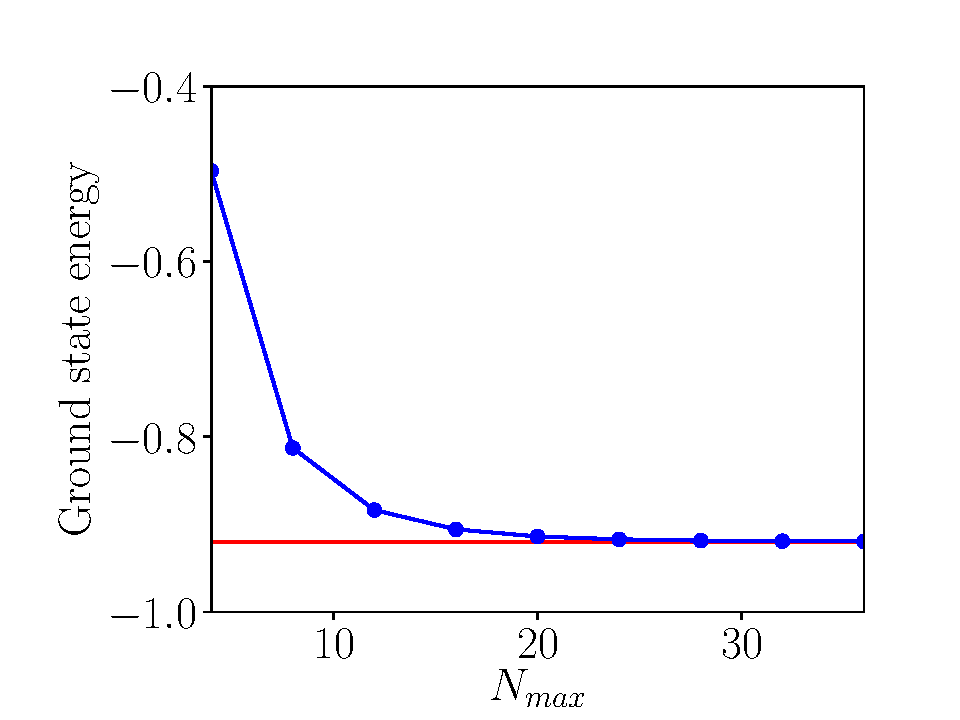
\includegraphics[width=0.5\linewidth]{alpha_2body_nmax}}
\subfloat[$\hat{V}_\beta$\label{fig:2body_b_nmax}]{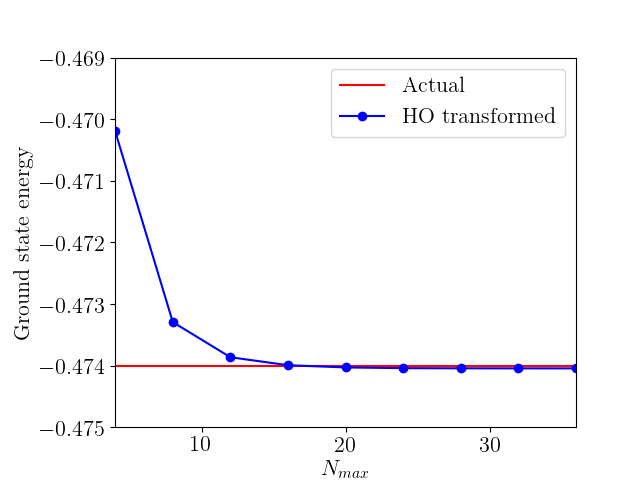
\includegraphics[width=0.5\linewidth]{beta_2body_nmax}}
\end{center}
\caption{2-body harmonic oscillator basis convergence patterns for (a) $\hat{V}_\alpha$ and (b) $\hat{V}_\beta$ with respect to $N_{max}$.}
\label{fig:2body_nmax}
\end{figure}

To lay the groundwork for exploring the 3-body system, we transform our 2-body operators into a symmetric harmonic oscillator basis. In practice, we truncate our harmonic oscillator basis at some maximum total harmonic oscillator number, $N_{max}$. We use $N_{max}=28$, and we show in Fig.~\ref{fig:2body_nmax} that by this value the 2-body ground state eigenvalue is converged to the value calculated in momentum space to within 0.1\%.

\begin{figure}[t]
\begin{center}
\subfloat[$\hat{T}$ transformed\label{fig:kin_e_transformed}]{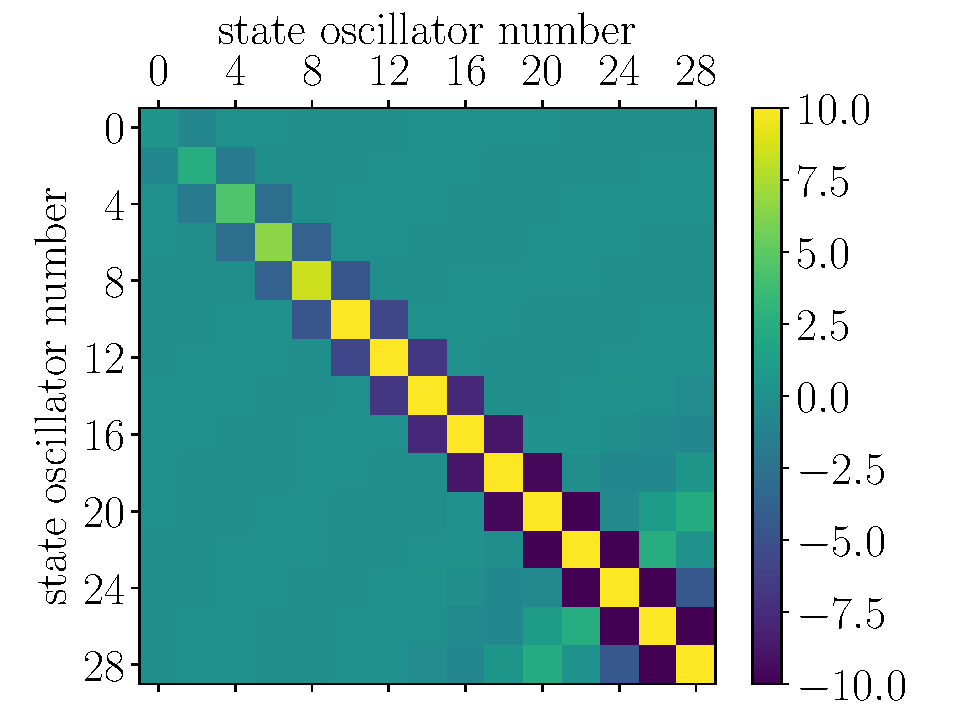
\includegraphics[trim={0 0 4cm 0},clip,width=0.43\linewidth]{transform_kin_e}}
\subfloat[$\hat{T}$ from HO basis\label{fig:kin_e_ho}]{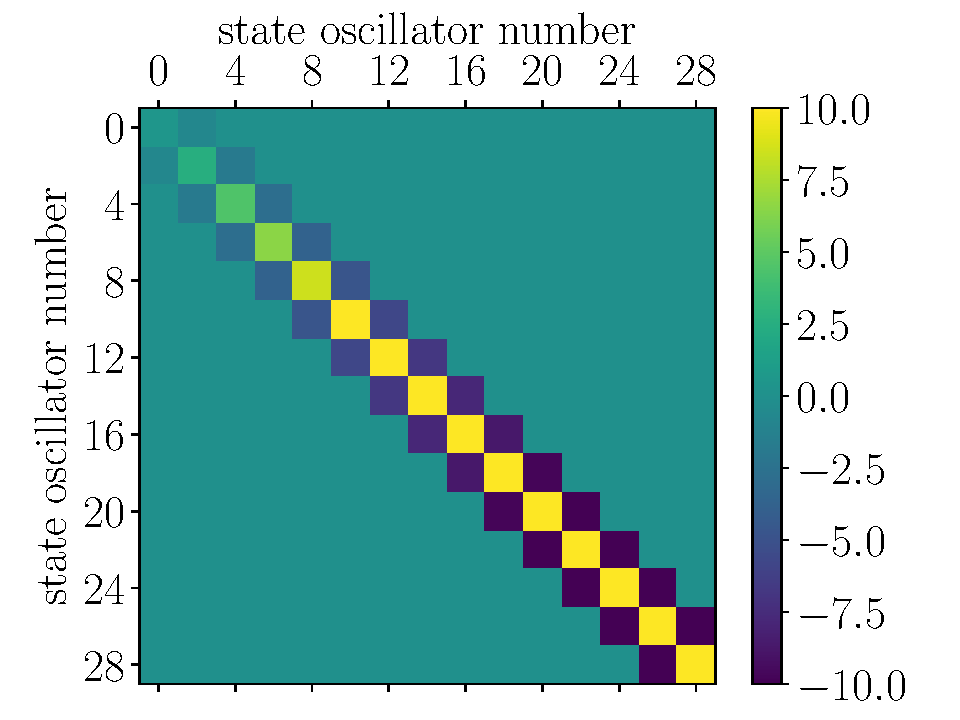
\includegraphics[trim={0 0cm 0 0},clip,width=0.57\linewidth]{pure_kin_e}}
\end{center}
\caption{The harmonic oscillator kinetic energy operator as computed (a) via a transformation from the momentum space operator and (b) directly from the harmonic oscillator basis.}
\label{fig:2body_kin_comp}
\end{figure}

As an additional check, we compare the kinetic energy calculated in momentum space and transformed to harmonic oscillator space to the kinetic energy operator computed directly from the symmetric harmonic oscillator basis. We find in Fig.~\ref{fig:2body_kin_comp} that they are the same at low harmonic oscillator number, which corresponds to low energies. As these are the same, for the 3-body case we will be working with the transformed potential and the kinetic energy computed directly from the harmonic oscillator basis, as it is cleaner to calculate.%At high energies, we see the transform kinetic energy operator stray from the true tridiagonal form of the kinetic energy in harmonic oscillator space. This is caused by ringing due to the truncation of the harmonic oscillator basis. However, this ringing does not affect the low-energy parts of the kinetic energy and thus has no effect on the lowest eigenvalues, the bound state energies we care about preserving. 

\section{3-Body}

For the 3-body system, the key results for us to reproduce are the 3-body ground state energies in Table \ref{table:negele_params} and the induced 3-body force in Fig.~\ref{fig:jurg_vfull} for $\hat{G}_s=\hat{T}$.

\subsection{3-Particle Ground State}

For the 3-body symmetric harmonic oscillator basis, we stay with $N_{max}=28$ in order to replicate the same results as Ref.~\cite{Jurgenson:2008jp}. There is also a performance consideration here, because, while the basis size for a 2-body system scales linearly in $N_{max}$, the basis size for a 3-body system scales quadratically in $N_{max}$. Since at $N_{max}=28$ we are already converged to within 1\% in the 3-body system, as shown in Fig.~\ref{fig:3body_nmax}, by raising $N_{max}$ we would simply be slowing down our ability to test alternative flow generators without any substantial numerical gain. With $N_{max}=28$, we get the 3-body ground state energy to be $-2.563$ for $\hat{V}_\alpha$ and $-1.708$ for $\hat{V}_\beta$, matching the values listed in Table \ref{table:negele_params}.

\begin{figure}[th!]
\begin{center}
\subfloat[$\hat{V}_\alpha$\label{fig:3body_a_nmax}]{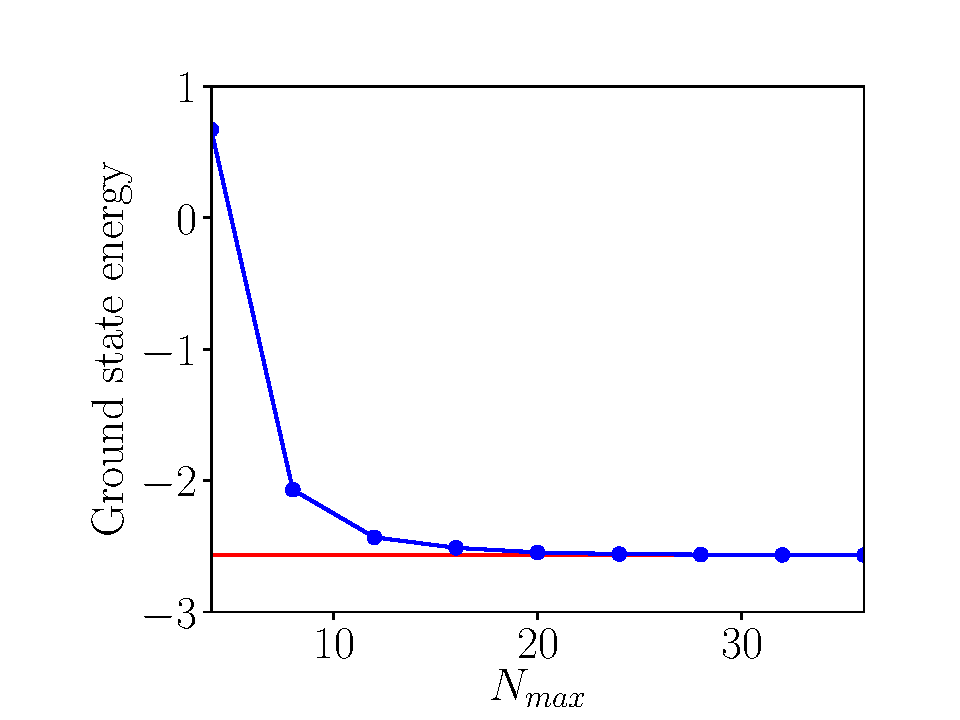
\includegraphics[width=0.5\linewidth]{alpha_3body_nmax}}
\subfloat[$\hat{V}_\beta$\label{fig:3body_b_nmax}]{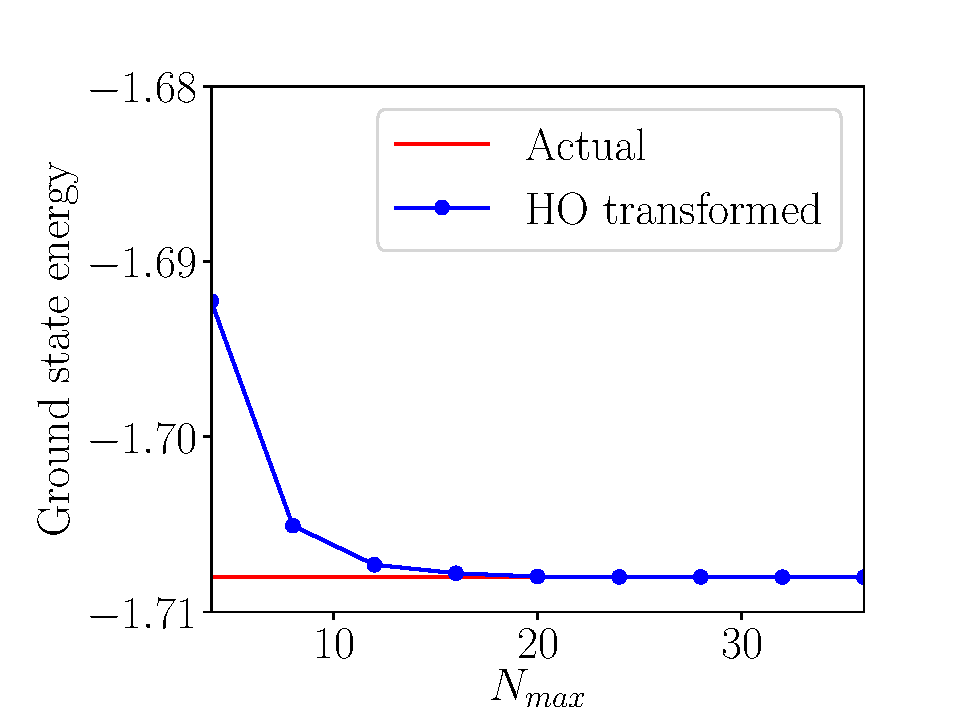
\includegraphics[width=0.5\linewidth]{beta_3body_nmax}}
\end{center}
\caption{3-body harmonic oscillator basis convergence patterns for (a) $\hat{V}_\alpha$ and (b) $\hat{V}_\beta$ with respect to $N_{max}$.}
\label{fig:3body_nmax}
\end{figure}
\begin{figure}[th!]
\begin{center}
\subfloat[2-body ground state energy\label{fig:2body_a_w}]{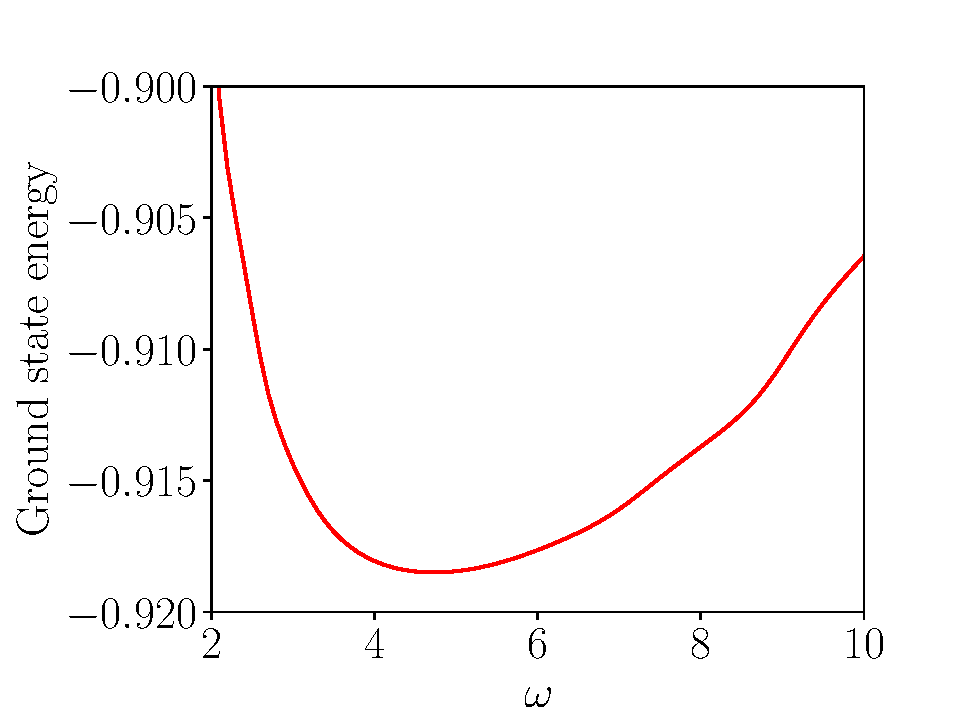
\includegraphics[width=0.5\linewidth]{alpha_2body_w}}
\subfloat[3-body ground state energy\label{fig:3body_a_w}]{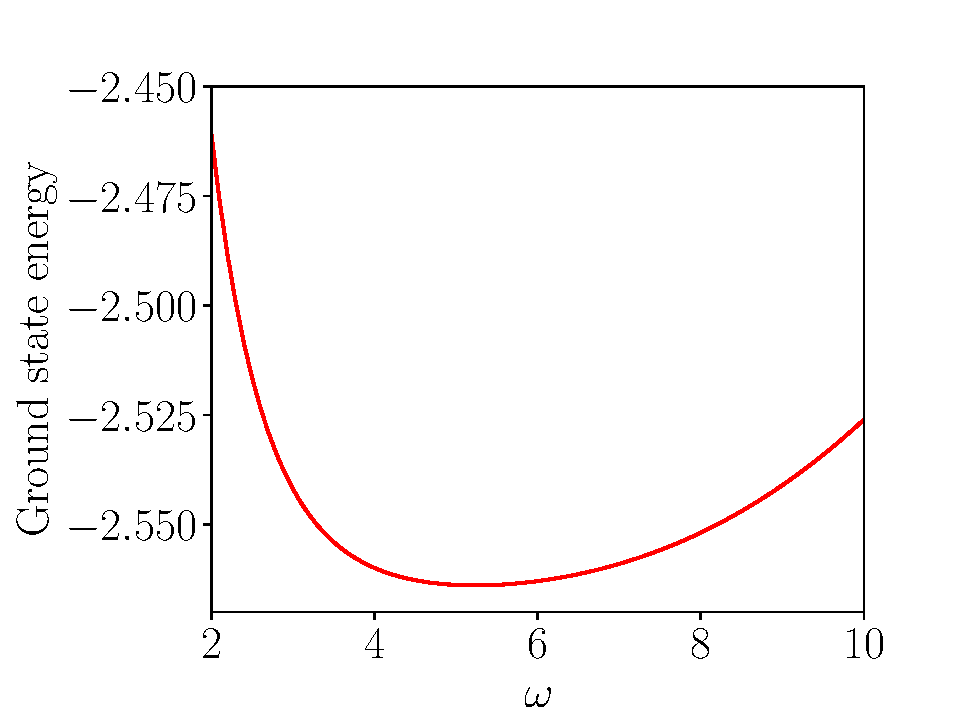
\includegraphics[width=0.5\linewidth]{alpha_3body_w}}
\end{center}
\caption{Ground state energy is a smooth function of $\omega$ and thus easy to minimize.}
\label{fig:alpha_w}
\end{figure}

When going from momentum space to harmonic oscillator space, we must optimize $\omega$, the parameter for the harmonic oscillator basis. The optimal $\omega$ will minimize the ground state energy, which will be the best we can do to reproduce the low-energy eigenvalues for a given $N_{max}$. We find that roughly the same value for $\omega$ optimizes both the 2-body ground state energy and the 3-body ground state energy, as shown in Fig.~\ref{fig:alpha_w}.


\subsection{3-Body Force Induction for $\hat{G}_s=\hat{T}$}

We then compare the 3-body ground state values for a Hamiltonian evolved in 3-body systems and a Hamiltonian evolved in the 2-body system and embedded in the 3-body system at each intermediate point during the evolution. We see in Fig.~\ref{fig:heinz_vfull} the same trends as in Fig.~\ref{fig:jurg_vfull}. With this, we have verified the correctness of our framework up to the 3-body system and can now use it to test the 3-body force induction of SRG with alternative flow operators.

\begin{figure}[t]
\begin{center}
\subfloat[$\hat{V}_\alpha$\label{fig:heinz_va}]{\centering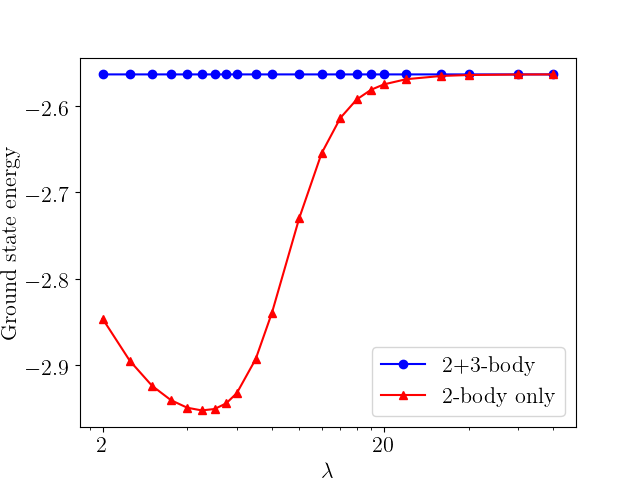
\includegraphics[width=0.5\linewidth]{manybody_T_alpha}}
\subfloat[$\hat{V}_\beta$\label{fig:heinz_vb}]{\centering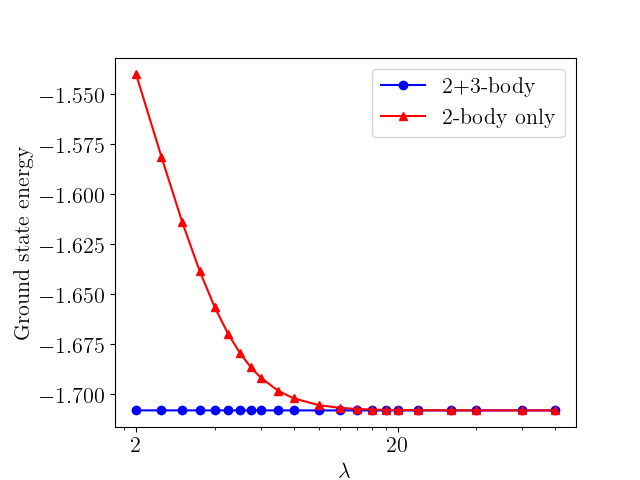
\includegraphics[width=0.5\linewidth]{manybody_T_beta}}
\end{center}
\caption{3-body force induction with $\hat{G}_s=\hat{T}$ leading to error in the computed 3-body ground state energy.}
\label{fig:heinz_vfull}
\end{figure}

\subsection{3-Body Force Induction for Alternative Flow Operators}

We test two parametrizations for an alternative flow operator, $\hat{H}_{BDHO}$, that is block diagonal in harmonic oscillator space, defined as
\begin{equation}
\hat{G}_s = \hat{H}_{BDHO} = \hat{T} + \hat{V} \Theta(N - \Lambda) \Theta(N' - \Lambda),
\end{equation}
where $\Lambda$ is the block cutoff in harmonic oscillator space. We use $\Lambda=6$ and $\Lambda=10$ for our tests. We find that both parametrizations offer a substantial decrease in the induced 3-body force, as shown in Fig.~\ref{fig:heinz_newfull}. In particular, $\Lambda=10$ induces nearly no 3-body force, keeping the 3-body ground state energy within less than 1\% of its true value.

\begin{figure}[th!]
\begin{center}
\subfloat[$\hat{V}_\alpha$\label{fig:heinz_newa}]{\centering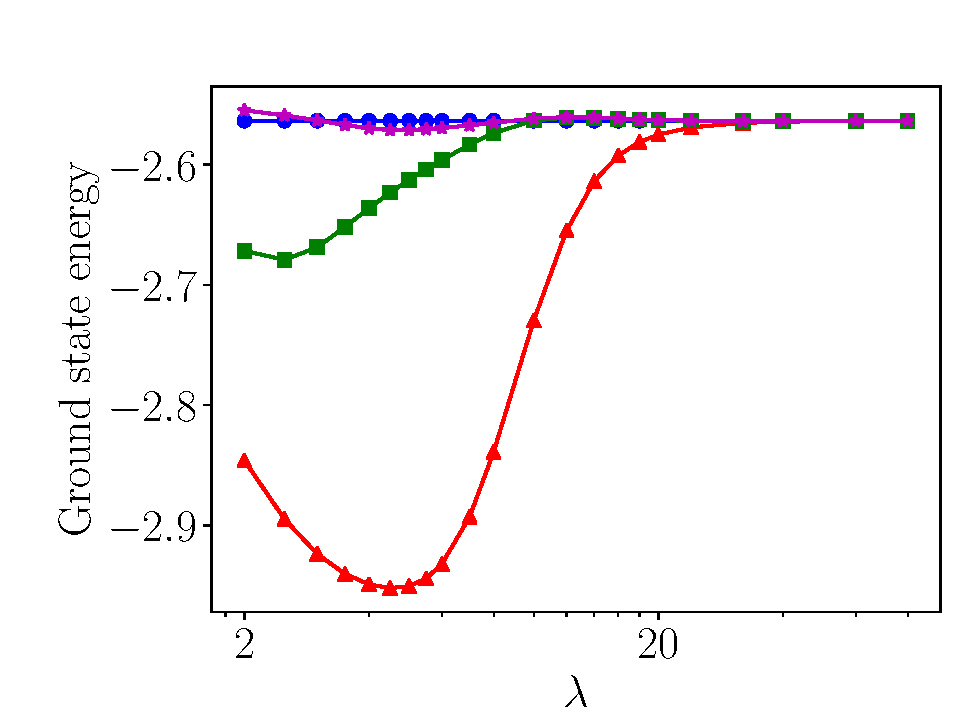
\includegraphics[width=0.5\linewidth]{new_alpha}}
\subfloat[$\hat{V}_\beta$\label{fig:heinz_newb}]{\centering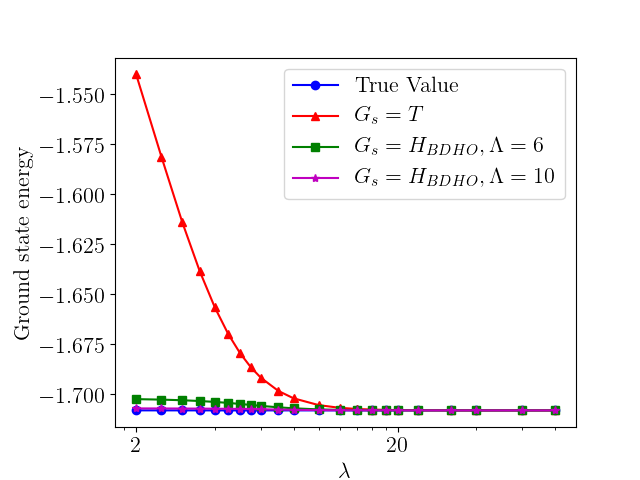
\includegraphics[width=0.5\linewidth]{new_beta}}
\end{center}
\caption{3-body force induction for various different generators. We see $\hat{H}_{BDHO}$ leads to a generally smaller induced 3-body force.}
\label{fig:heinz_newfull}
\end{figure}

While these results show promise for $\hat{H}_{BDHO}$ as an improved flow operator, they are still preliminary. It may be the case case that $\hat{H}_{BDHO}$ and $\hat{T}$ decouple off-diagonal matrix elements at different rates with respect to $\lambda$, meaning that $\lambda=1$ for $\hat{T}$ evolutions does not correspond to $\lambda=1$ for $\hat{H}_{BDHO}$ evolutions. While some quick tests ``by eye" suggest this is not the case, it must still be verified more robustly. This can be done by imposing some cutoff on the 2-body space and checking that the $\lambda$ at which both evolutions reproduce the correct ground state energy is similar. If it is not similar, it will be necessary to figure out a mapping of corresponding values of $\lambda$ for the two evolutions.

Additionally, tests must be run that look at 4-body and 5-body forces, in order to ensure induced many-body forces remain strictly smaller than for $\hat{G}_s=\hat{T}$. The \texttt{srg1d} framework also allows to easily test more flow operators, which we must due to get a more comprehensive idea of what features of the flow operators reduce or enhance many-body force induction.



\chapter{Conclusion and Outlook}

\section{Future Development on \texttt{srg1d}}

\section{Conclusion}

\section{Open Questions and Outlook}


\backmatter
% We use BIBTeX for the bibliography---you don't have to
\bibliographystyle{unsrt} % use your favorite BIBTeX style
% \nocite{*} % To display all refs, even uncited refs (useful when editting)
\bibliography{thesisbib}

% If for some reason you are anti-BIBTeX, then you would use the
% following instead of the above:
%\begin{thebibliography}{99}
% ...
%\end{thebibliography}


% Note: GS 2010 requires bibliography/references _before_ the appendix
% if you believe their guidelines; however, conversations with GS
% staff suggests _they don't care_. Go figure. So do what you like.

\appendix
% \chapter{My Appendix needs to be removed...}


A citation~\cite{bib2}. \lipsum[1]

\section{Sections in an Appendix, What is the World Coming to?}

Another citation~\cite{bib1}.  \lipsum[1]
\begin{equation}
\frac{1}{\sqrt{2\pi \sigma^2}}e^{-\frac{1}{2}(\frac{x-\mu}{\sigma})^2}
\end{equation}
\lipsum[1]

\subsection{Subsections, Too!}

\lipsum[2-5]
\begin{equation}
e^{i\pi} + 1 = 0
\end{equation}
\lipsum[1-3]

% \chapter{I don't feel so good}

\lipsum


\end{document}
